\documentclass[pre,twocolumn,twoside,superscriptaddress,floatfix, aps, 10pt]{revtex4-1}

\usepackage{currfile}
\lefthyphenmin=3
\righthyphenmin=2

\usepackage{graphicx,epsfig,verbatim,enumerate}
\usepackage{amssymb,amsmath}
\usepackage{ifthen}

% Fonts and typesetting settings
\usepackage[sc]{mathpazo}
\usepackage[T1]{fontenc}
\linespread{1.05} % Palatino needs more space between lines
\usepackage{microtype}
\usepackage{textcomp}

\usepackage{longtable}

\usepackage{mathtools}

\newboolean{twocolswitch}

\newcommand{\www}[1]{\url{#1}}
\newcommand{\req}[1]{(\ref{#1})}
\newcommand{\Req}[1]{Eq.~(\ref{#1})}

% Lettrines
\usepackage{lettrine}

%useful shortcuts
\def\R{\ensuremath{\mathbb{R}}} %\ensuremath adds math mode, if forgotten
\def\Q{\ensuremath{\mathbb{Q}}}
\def\N{\ensuremath{\mathbb{N}}}
\def\Z{\ensuremath{\mathbb{Z}}}
\def\C{\ensuremath{\mathbb{C}}}

%shorcuts with arguments
\newcommand{\abs}[1]{\left\vert#1\right\vert} %nice absolute values
\newcommand{\bt}[1]{\textbf{#1}} %bold
\newcommand{\eq}[1]{\begin{align*}#1\end{align*}} %aligned equations
\newcommand{\norm}[1]{\left\lVert#1\right\rVert} %vector norm
\renewcommand{\eq}[1]{\begin{align*}#1\end{align*}} %aligned equations

%piecewise function

%\begin{displaymath}
%   f(x) = \left\{
%     \begin{array}{lr}
%       1 & : x \in \mathbb{Q}\\
%       0 & : x \notin \mathbb{Q}
%     \end{array}
%   \right.
%\end{displaymath} 


%environment
\newcommand{\tab}{\phantom{ssss}}

\usepackage{hyperref}
\usepackage{color}
\newcommand{\todo}[1]{\noindent\textcolor{blue}{{$\Box$ #1}}}

%colors
\definecolor{javagreen}{rgb}{0.25,0.5,0.35} %dark green color
\definecolor{lightblue}{rgb}{0.149,0.545,0.824} %solarized blue
\definecolor{sred}{rgb}{0.863, 0.196, 0.184} %solarized red

\newcommand{\blue}[1]{{\leavevmode\color{lightblue}{#1}}} %solarized blue 
\newcommand{\green}[1]{{\leavevmode\color{javagreen}{#1}}} %command for green
\newcommand{\red}[1]{{\leavevmode\color{sred}{#1}}} %solarized red
\newcommand{\gray}[1]{{\leavevmode\color[gray]{0.5}{#1}}} %gray text
\newcommand{\Prob}[1]{{\rm Pr}\left(#1\right)}


\setboolean{twocolswitch}{true}


\begin{document}

\title{\protect
Connecting every bit of knowledge: \\
The Structure of Wikipedia's first link network
}

\date{\today}

\author{
\firstname{Mark}
\surname{Ibrahim}
}
\email{mark.s.ibrahim@uvm.edu}

\affiliation{Department of Mathematics \& Statistics, 
    Computational Story Lab,  \\
    Vermont Complex Systems Center,
    Vermont Advanced Computing Core,
    The University of Vermont, Burlington, VT 05401.}

\author{
\firstname{Christopher}
\surname{M. Danforth}
}
\email{chris.danforth@uvm.edu}

\affiliation{Department of Mathematics \& Statistics, 
    Computational Story Lab,  \\
    Vermont Complex Systems Center,
    Vermont Advanced Computing Core,
    The University of Vermont, Burlington, VT 05401.}

\author{
\firstname{Peter}
\surname{Sheridan Dodds}
}

\email{peter.dodds@uvm.edu}

\affiliation{Department of Mathematics \& Statistics, 
    Computational Story Lab,  \\
    Vermont Complex Systems Center,
    Vermont Advanced Computing Core,
    The University of Vermont, Burlington, VT 05401.}


\begin{abstract}
  \protect
Apples, porcupines, and the most obscure Dylan song---is every topic a few clicks from Philosophy? 
Within Wikipedia, the surprising answer is yes: nearly all 
paths lead to Philosophy.
Wikipedia is the largest, most meticulously indexed collection of human knowledge ever amassed. 
More than information about a topic, Wikipedia is a web of naturally emerging relationships.  
By following the first link in an article, we connect entries to form a directed network: Wikipedia's First Link Network. 
Here, we study the English edition of Wikipedia's First Link Network for insight into how the many topics, ideas, people, objects, and events
are related and organized.  
We algorithmically parse all 4.7 million articles to construct a map of Wikipedia's First Link Network. 
We traverse every possible path through the network, 
measuring the accumulation of first links, path lengths, basins, cycles, and the influence a particular article exerts in shaping the 
network.
We discover many scale-free distributions, find Philosophy at a salient center, and uncover a flow from specific to general 
culminating around fundamental notions such as Community, State, and Science. 
Curiously, we also observe a gravitation towards topical articles including Health Care and Fossil Fuel.
These findings enrich our view of how we connect and structure
Wikipedia's ever growing store of knowledge.
 
\end{abstract}

\maketitle

TODO: 
* fix end of second paragraph in Results Section
    * power-law biz and total peter is asking for
* fix exponent reporting (with alpha) 
    * figure out what gamma size freq means

\section{Traversing the First Link Network}

An essential feature of a directed network's structure is the degree distribution 
\cite{newman}. 
The degree distribution has been used to study many phenomena from disease outbreak 
\cite{disease} 
to the dynamics of social networks 
\cite{social_nets}.
The in-degree distribution in the FLN describes how many first links point to a 
particular article. 
We measure the in-degree in the FLN to gauge the number of articles referencing a particular article.
Articles with zero in-degree have no references---they are outer leaves in the FLN. 
Similar to PageRank, the in-degree 
provides a way to rank the articles in Wikipedia, allowing us to see 
whether authors tend to reference all articles equally or only a few.


Our greater interest is lies in the richer dynamics of how many articles fit together---how links create a flow through the FLN.
We construct a path through the FLN with each article 
leading to the next through the first link. 
For example ``Train'' has a first link to ``Conveyance of Passengers and Goods,'' which is itself
an article with a first link to ``Goods'' and so on. 
As shown in Fig.~\ref{fig:Train First Links}, the path starting at ``Train'' 
contains ``Goods,'' ``Economics,'' ``Social Science,''
ultimately leading to ``Philosophy''.

\begin{figure*}[tp!]
  \centering	
  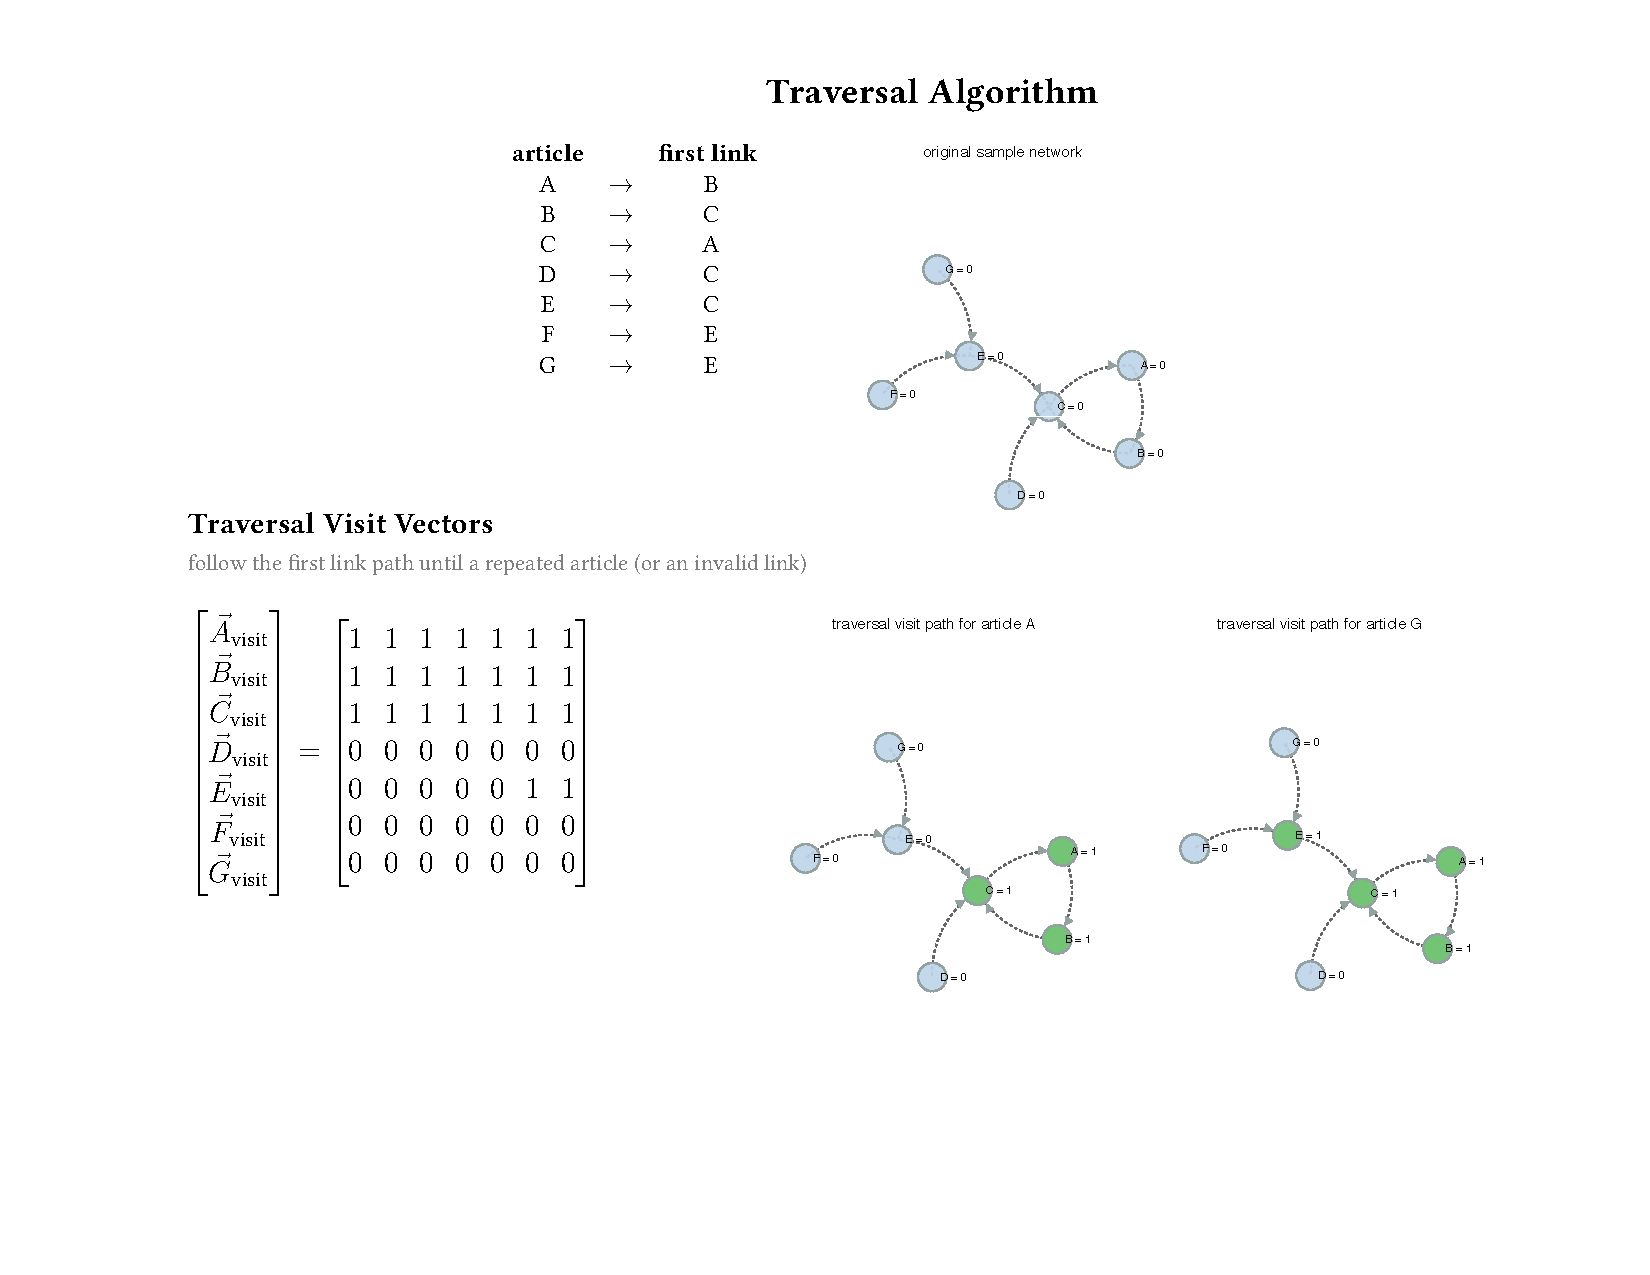
\includegraphics[width=\textwidth]{graphics/traversal_visit_algo_figure.pdf}  
  \caption{
    \textbf{Traversal Visit Algorithm on a sample network.}
     The traversal visit vectors are an adjacency matrix for the paths through the network: the first column is indicates the path formed starting with article A. The number of traversal visits for article A is then the number of paths containing A or the sum of the first row in our matrix:
     $\sum_{i=1}^7 A_{\text{visit, i}} = 7$.
  }
  \label{fig:Traversal Visits}
\end{figure*}

Starting at each article, we construct a path through the FLN, 
ultimately mapping a flow of connections among articles.
The method is order agnostic with respect to which articles are selected first. As long as each article is selected eventually, the resulting metrics are equivalent.

We use the notion of a path through the FLN to describe 
the structure of the FLN as a flow relating topics. 
Grounded in the dynamics of river networks
\cite{geo_basins},
we characterize features of the FLN as a flow through first links.
Previous studies have used flow to characterize the structure of river networks
\cite{dodds} and describe the organization of food systems as transportation networks
\cite{food_webs}.
With paths to mark flow through the FLN, we develop metrics to 
gauge the accumulation of references, 
the length of the path relating articles, and the influence a particular
article exerts in shaping the flow of links through the FLN.


The first metric we develop quantifies the accumulation of first links.
The algorithm begins by selecting an article, then traversing the path formed
by following the first links. Each time a first link references an article, we increment a count
associated with the article. 
We continue until the first link is retraced or is invalid---defined here to mean outside of Wikipedia.
We select a second article and repeat the process until we have 
constructed a path for each article in the network. We call the resulting count for each article the number of {\it traversal visits}. The number of traversal visits of an article 
measures the number of references flowing to the ideas in the article---equivalent
to basin area in geomorphology. 

\begin{figure}[tp!]
  \centering	
  \includegraphics[width=\columnwidth]{graphics/traversal_funnel_algo_figure.pdf}
  \caption{
    \textbf{Traversal Funnel Algorithm on a sample network.}
  The algorithm for traversal funnels is identical to the previous algorithm for traversal visits with one alteration: the path ends at the start of a cycle to distinguish articles directing a path into a cycle from articles that simply happen to be in a highly traversed path. We can construct similar vectors by considering each path through the network, measuring traversal funnels for a particular article as the sum of the entries in its corresponding row. For example
  the number of traversal funnels for article $E$ is 
  $\sum_{i=1}^7 E_{\text{funnel, i}} = 2$.}
  \label{fig:Traversal Funnels}

\end{figure}

We can characterize the paths in the FLN as a matrix with each column corresponding to a path. In our sample network 
(Fig.~\ref{fig:Traversal Visits}), the path starting at article A is the 
first column in the traversal visits matrix. 
An entry of $1$ indicates the path contains a given article and 
$0$ indicates the path does not.
To compute the number of traversal visits for an article, we sum the corresponding row in our matrix.
The traversal visits matrix for 
our Wikipedia dataset consists of 121 million entries to account for each path through the FLN. 

By measuring the number of first links between
two articles, we obtain an additional piece of information we call 
{\it path length.} We can compute the length of a path by summing 
along a column in our traversal visits matrix. 
In our Wikipedia dataset, the sum of all path lengths is 232 million first links.
The path length describes how closely related topics are.
The greater the number of first links separating two articles, the greater the number of ideas needed to relate their corresponding ideas. Although
``Train'' is related to ``Economics'' for example, there are several articles
bridging the connection:
``Train'' is more specifically related to transportation, whose object
is often goods. Goods are one of the fundamental objects of study in Economics.
Described in links, this relationship is captured by a relatedness of $4$ 
first links ultimately connecting ``Train'' to ``Economics.'' 

One possible path through the FLN is a {\it cycle} or a group of articles 
linking to one another inside a loop. In our sample network 
(Fig.~\ref{fig:Traversal Visits}) 
a 3-cycle exists among nodes A, B, and C. 
We can readily identify
the types of cycle structures within the FLN
and rank each by 
the number of references directed towards a cycle. 


We can also form and rank {\it basins} in the network by identifying groups of 
path-connected articles, not necessarily forming a perfect cycle.
A basin connects a group of articles and identifies the paths 
to a particular article.

While traversal visits measure accumulation, each article's first link also 
influences the shape of the FLN. 
At a large point of accumulation, a single article's first link 
can exert great influence over the shape of the FLN by directing many
references on a particular path. To distinguish between an article 
that simply happened to fall within a cycle from an article funneling 
many first links, we develop a second metric called {\it traversal funnels}.

To measure traversal funnels, we traverse the FLN in the same manner as we 
did for traversal visits, but end a path once we enter a cycle.
We are then able to distinguish between an article related to many other ideas
only by virtue of its place in a cycle, from an article exerting influence over where the first links flow. 
An article with a large number of traversal funnels directs many references
into a particular cycle. In our sample network 
(see figure~\ref{fig:Traversal Funnels}) article C 
directs the flow of links towards the 3-cycle, while articles A and B are 
recipients of the flow---without exerting any direct influence themselves. 

By studying the FLN not only as collection of directly linked pairs of articles, but
as a flow, 
we build a powerful arsenal of information.
From accumulated references, cycles, and basins, we can measure how the many articles in Wikipedia are organized and related.





\section{Results}

\subsection{Degree Distribution}

\begin{figure}[tp!]
  \centering	
  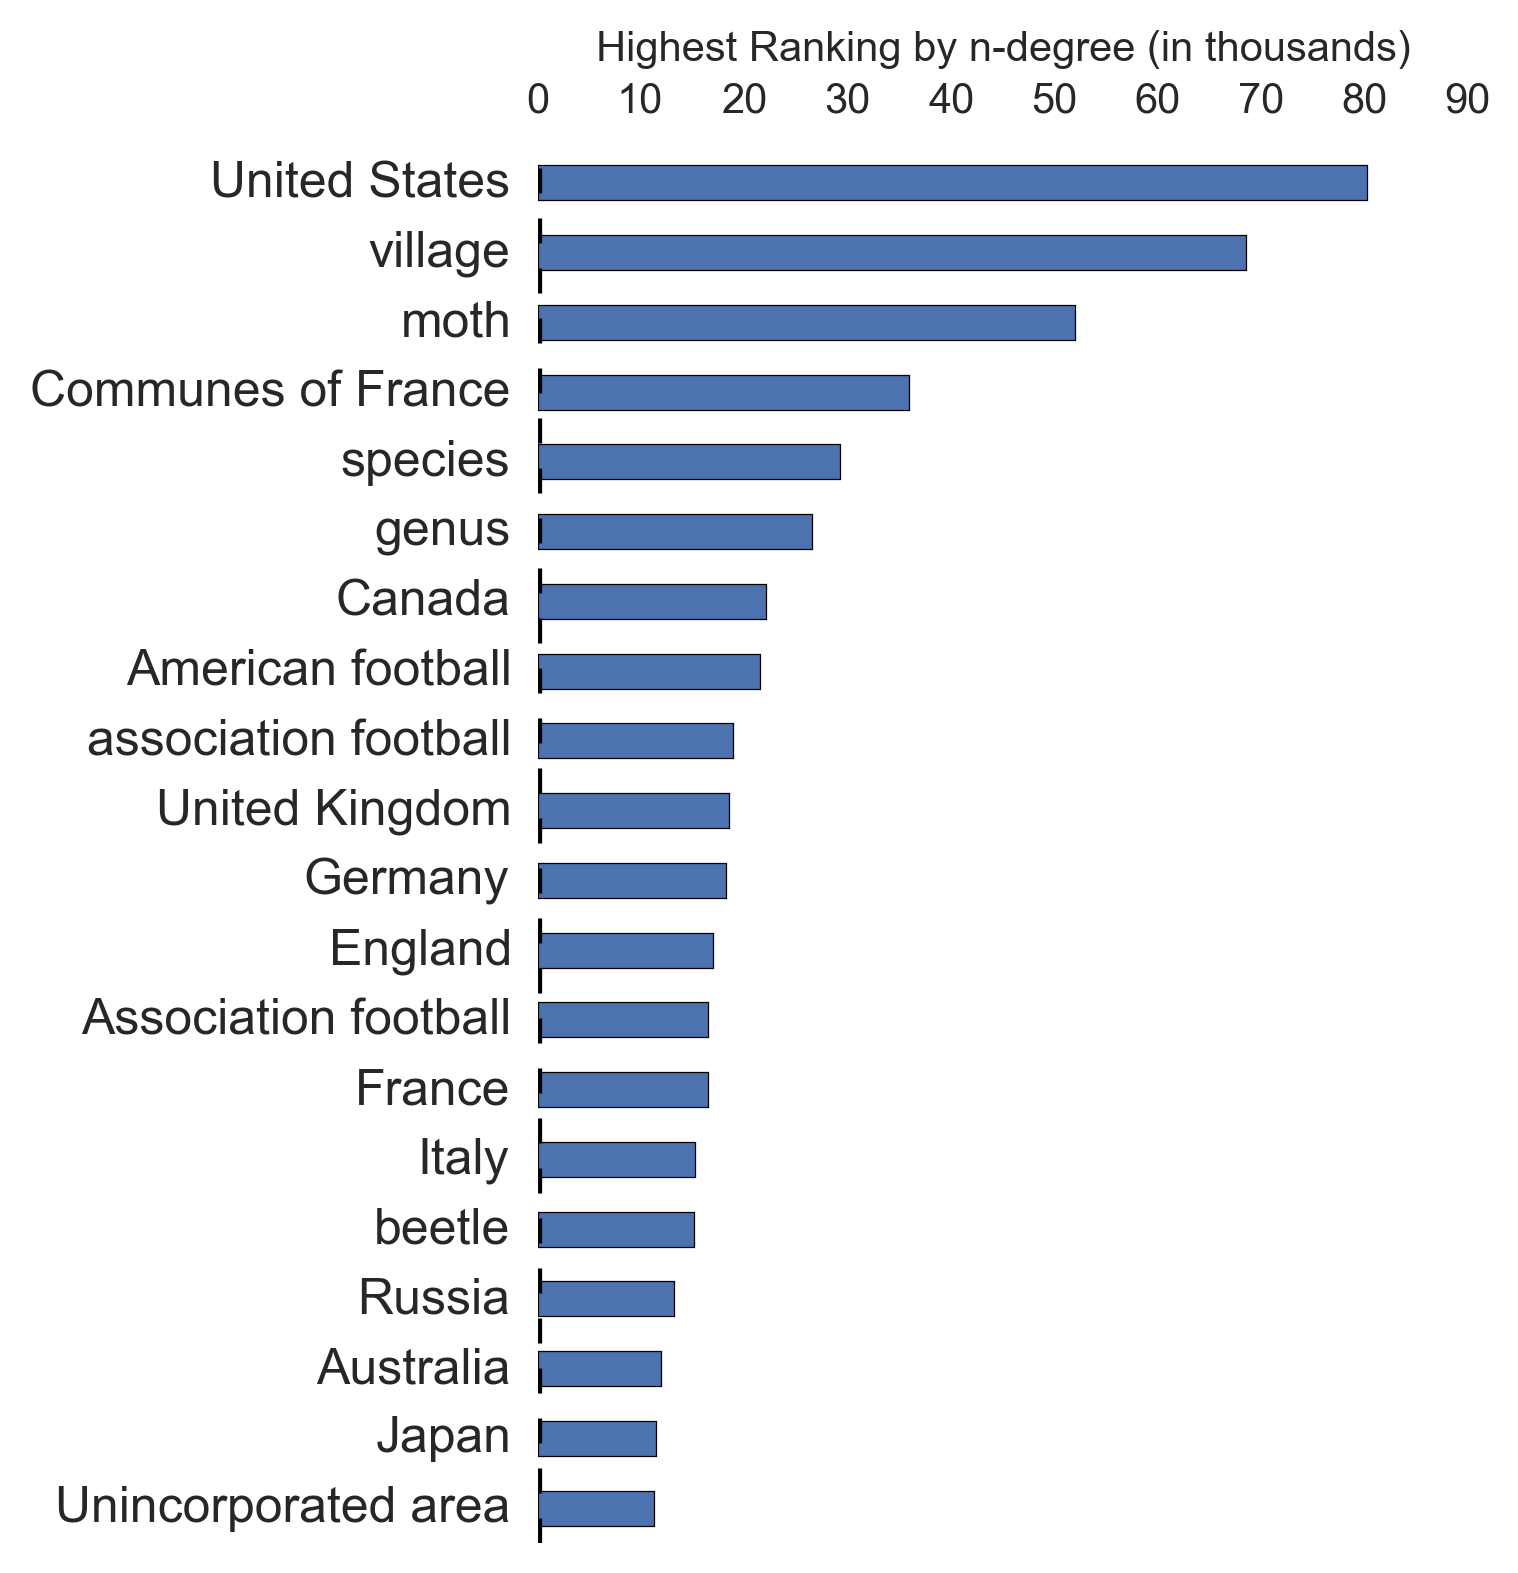
\includegraphics[width=\columnwidth]{graphics/articles_ndegree.png}
  \caption{
    \textbf{Highest Ranking Articles by in-degree.}
  }
  We rank each article by the number of direct first links to the article (in-degree). The highest-ranking articles tend to represent abstraction for concepts
  comprised of various facets.
  \label{fig:ndegree list}
\end{figure}

We rank all 11 million articles by in-degree to find 
the ``United States'' with 80,249 direct first links as the most referenced
Wikipedia article 
(Fig.~\ref{fig:ndegree list}). 
Other high-ranking articles
include foundational abstract concepts such as ``village,'' ``species,''; 
sports associations such as ``American Football,'' ``Association Football''; 
and developed nations such as ``France,'' ``Japan'', ``Russia,'' ``Australia,'' and 
the ``Netherlands.'' These high ranking articles are useful abstractions: nations
describe a collection of individuals with a common culture, language, or 
geographical proximity; sports teams describe an ever changing collection of 
sports players often associated with a cultural identity or a geographical 
region. 
Since abstractions such as nations and teams are inherently comprised
of many parts, authors reference the abstraction when describing a part.
In describing the New England Patriots or the New York Giants
for example, ``American Football'' is the natural abstraction, which 
anchors many specific teams.

``Philosophy'' and other philosophical concepts
are not among the highest-ranking articles by in-degree.
``Philosophy'' has an in-degree of only 581, with direct first links from articles about Philosophers and areas of Philosophy: ``Existentialism and Humanism,'' ``Predeterminism,'' ''Synoptic Philosophy,'' ``Qualia,'' ``Dorothy Emmet,'' and ``Christopher W. Morris.''
While many articles accumulate at ``Philosophy'' (see traversal visits discussion below), 
the accumulation is not the 
result of many articles directly referencing ``Philosophy.'' 
Instead, flows towards Philosophy as the 
ultimate anchor when generalizing from specific articles to broader notions.

\begin{figure}[tp!]
  \centering	
  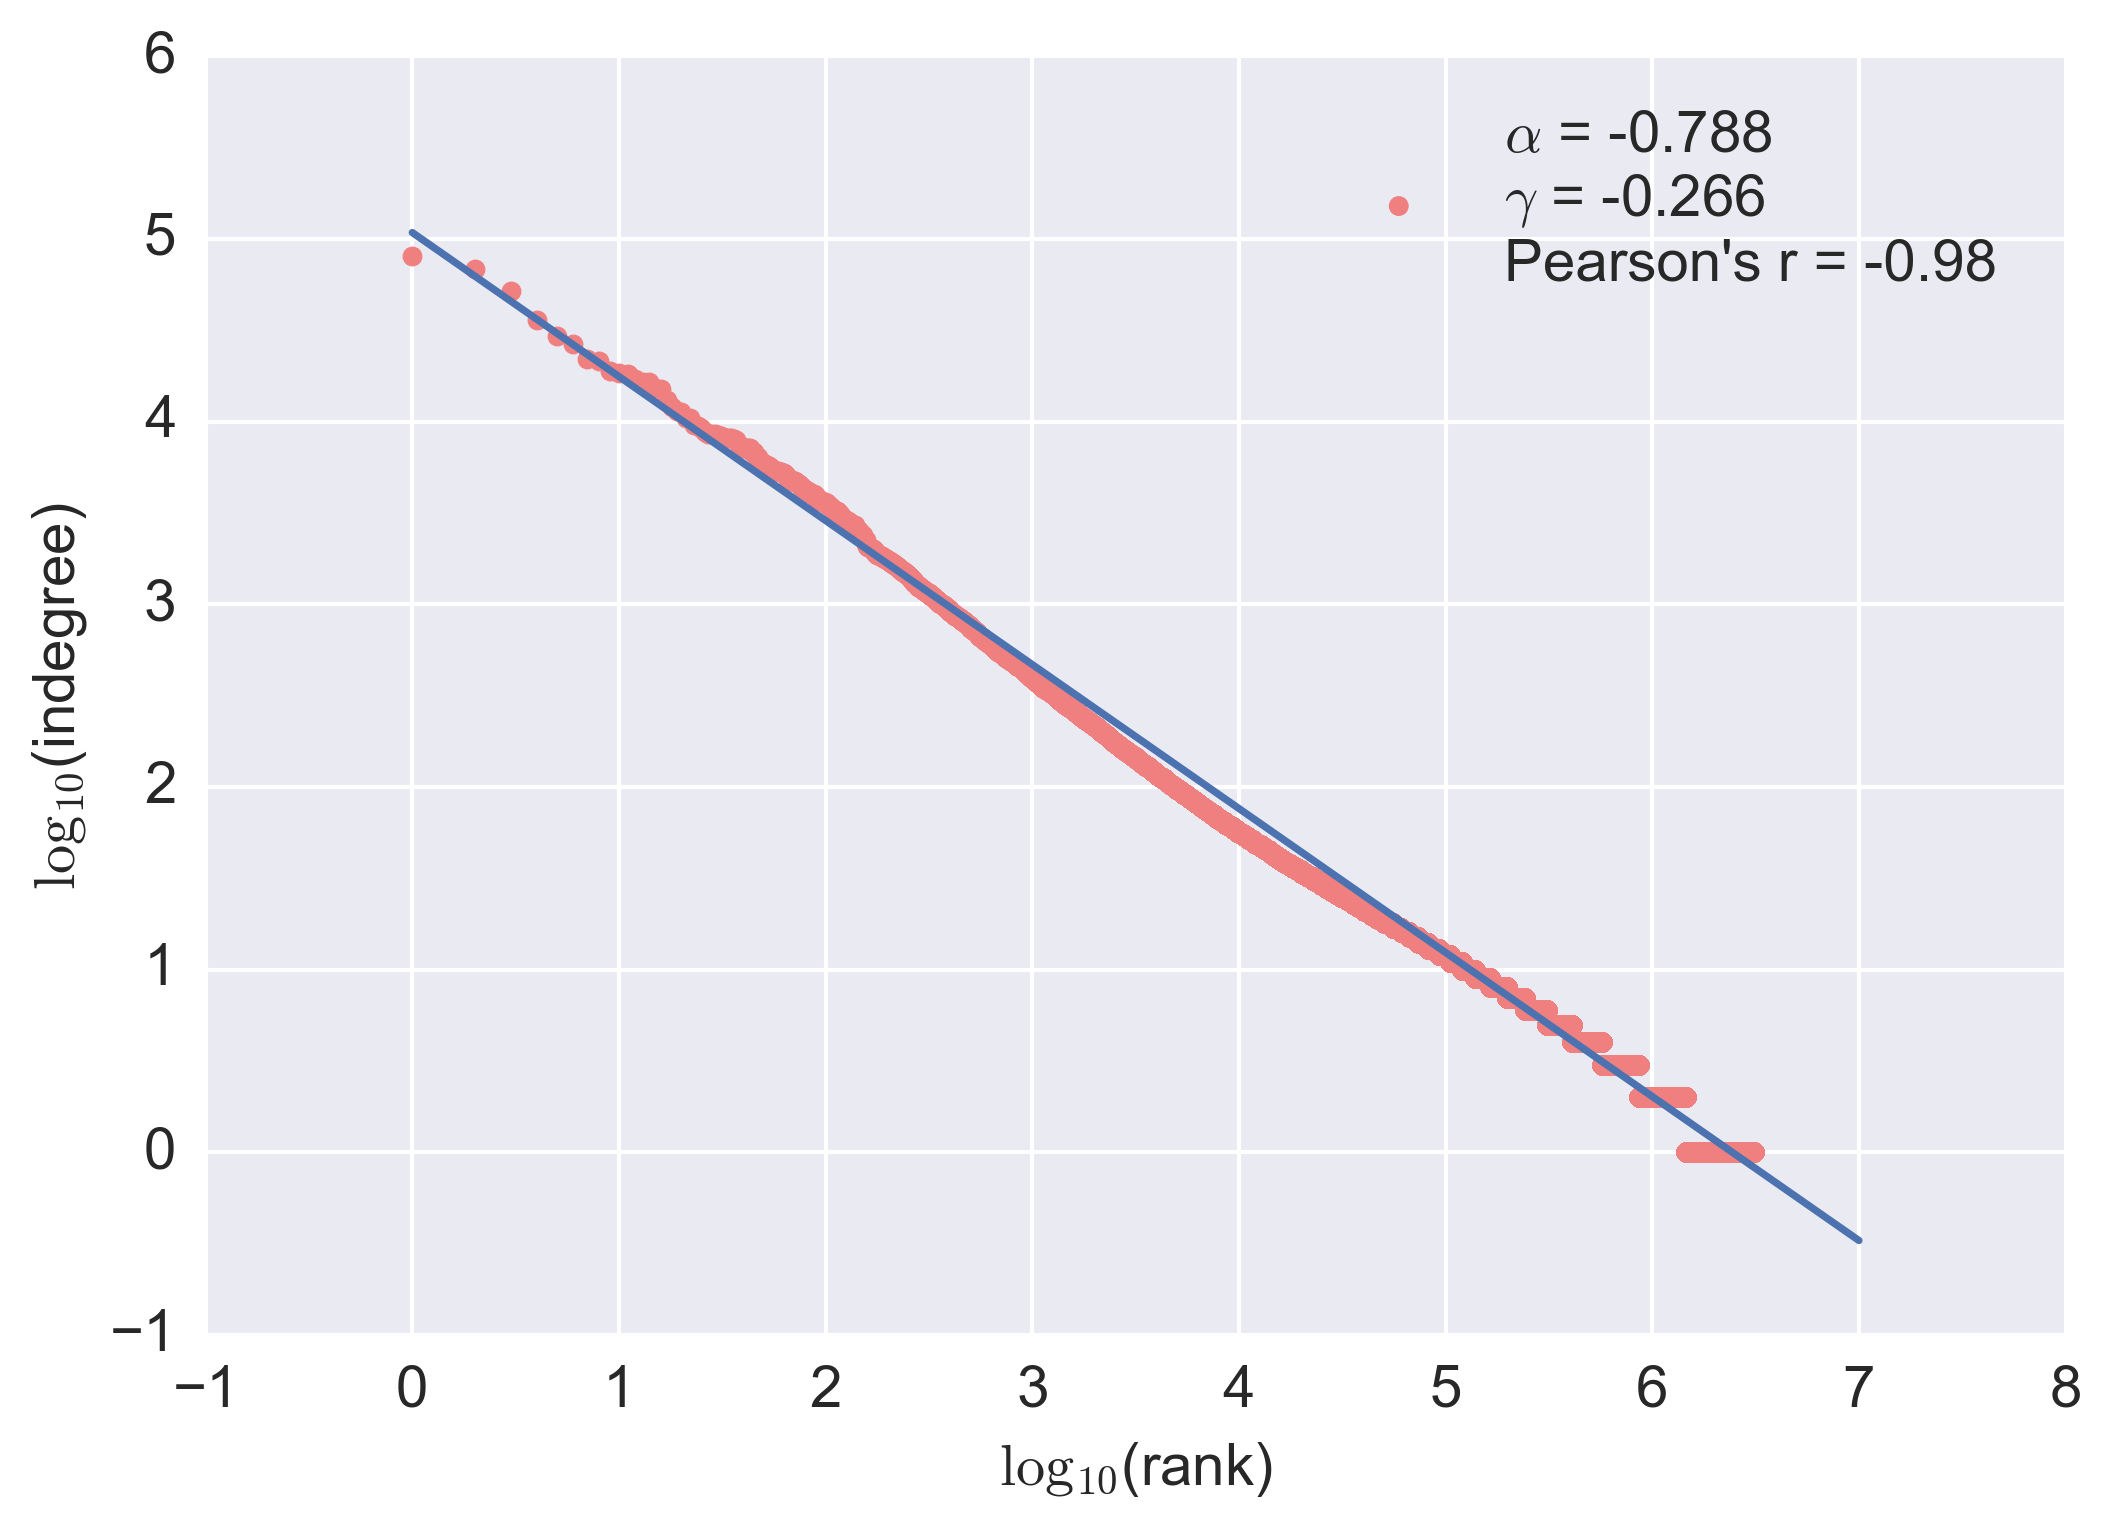
\includegraphics[width=\columnwidth]{graphics/ndegree_loglog.png}
  \caption{
    \textbf{FLN Degree Distribution.}
  }
  We construct a log-log plot and fit our results with a linear model. The result is a 
  an excellent fit with r = -0.98, yielding a power law exponent of -0.79. 
  The distribution appears to be scale free.
  \label{fig:degree distribution}
\end{figure}

The FLN's in-degree exhibits a decaying power-law distribution where a few articles 
receive most direct first references, while most articles receive few or none.
The average in-degree for all 11 million articles is 3.6 direct first links with a standard deviation of 89.5 links.
Only 4,826 articles have more than 100 direct first links and $75\%$ of articles
have fewer than 9. 
When fit with a linear model on a log-log scale (log(rank) versus log(in-degree)), 
the model's r value is $-0.98$ suggesting a strong log-log linear fit 
with a power law exponent of $-0.79$.\\



\subsection{Depth of the FLN}

We first seek to describe the depth of the FLN: how many links does a 
connection of among articles span? 
We find the longest path length is 365,
corresponding to the yearly calendar of Orthodox Liturgics.
Each day's Liturgics links to the next day's. On the last calendar day, the last article simply links back to January 1, forming a 365-cycle 
(see discussion of cycles).
We also find similarly lengthy paths following the evolution of a place or topic through time: 
``1953 in Scotland'' or ``1560s Architecture,'' with articles sequentially proceeding by year, decade or era.
In general, the longest paths connect temporally organized ideas.

\begin{figure}[tp!]
  \centering	
  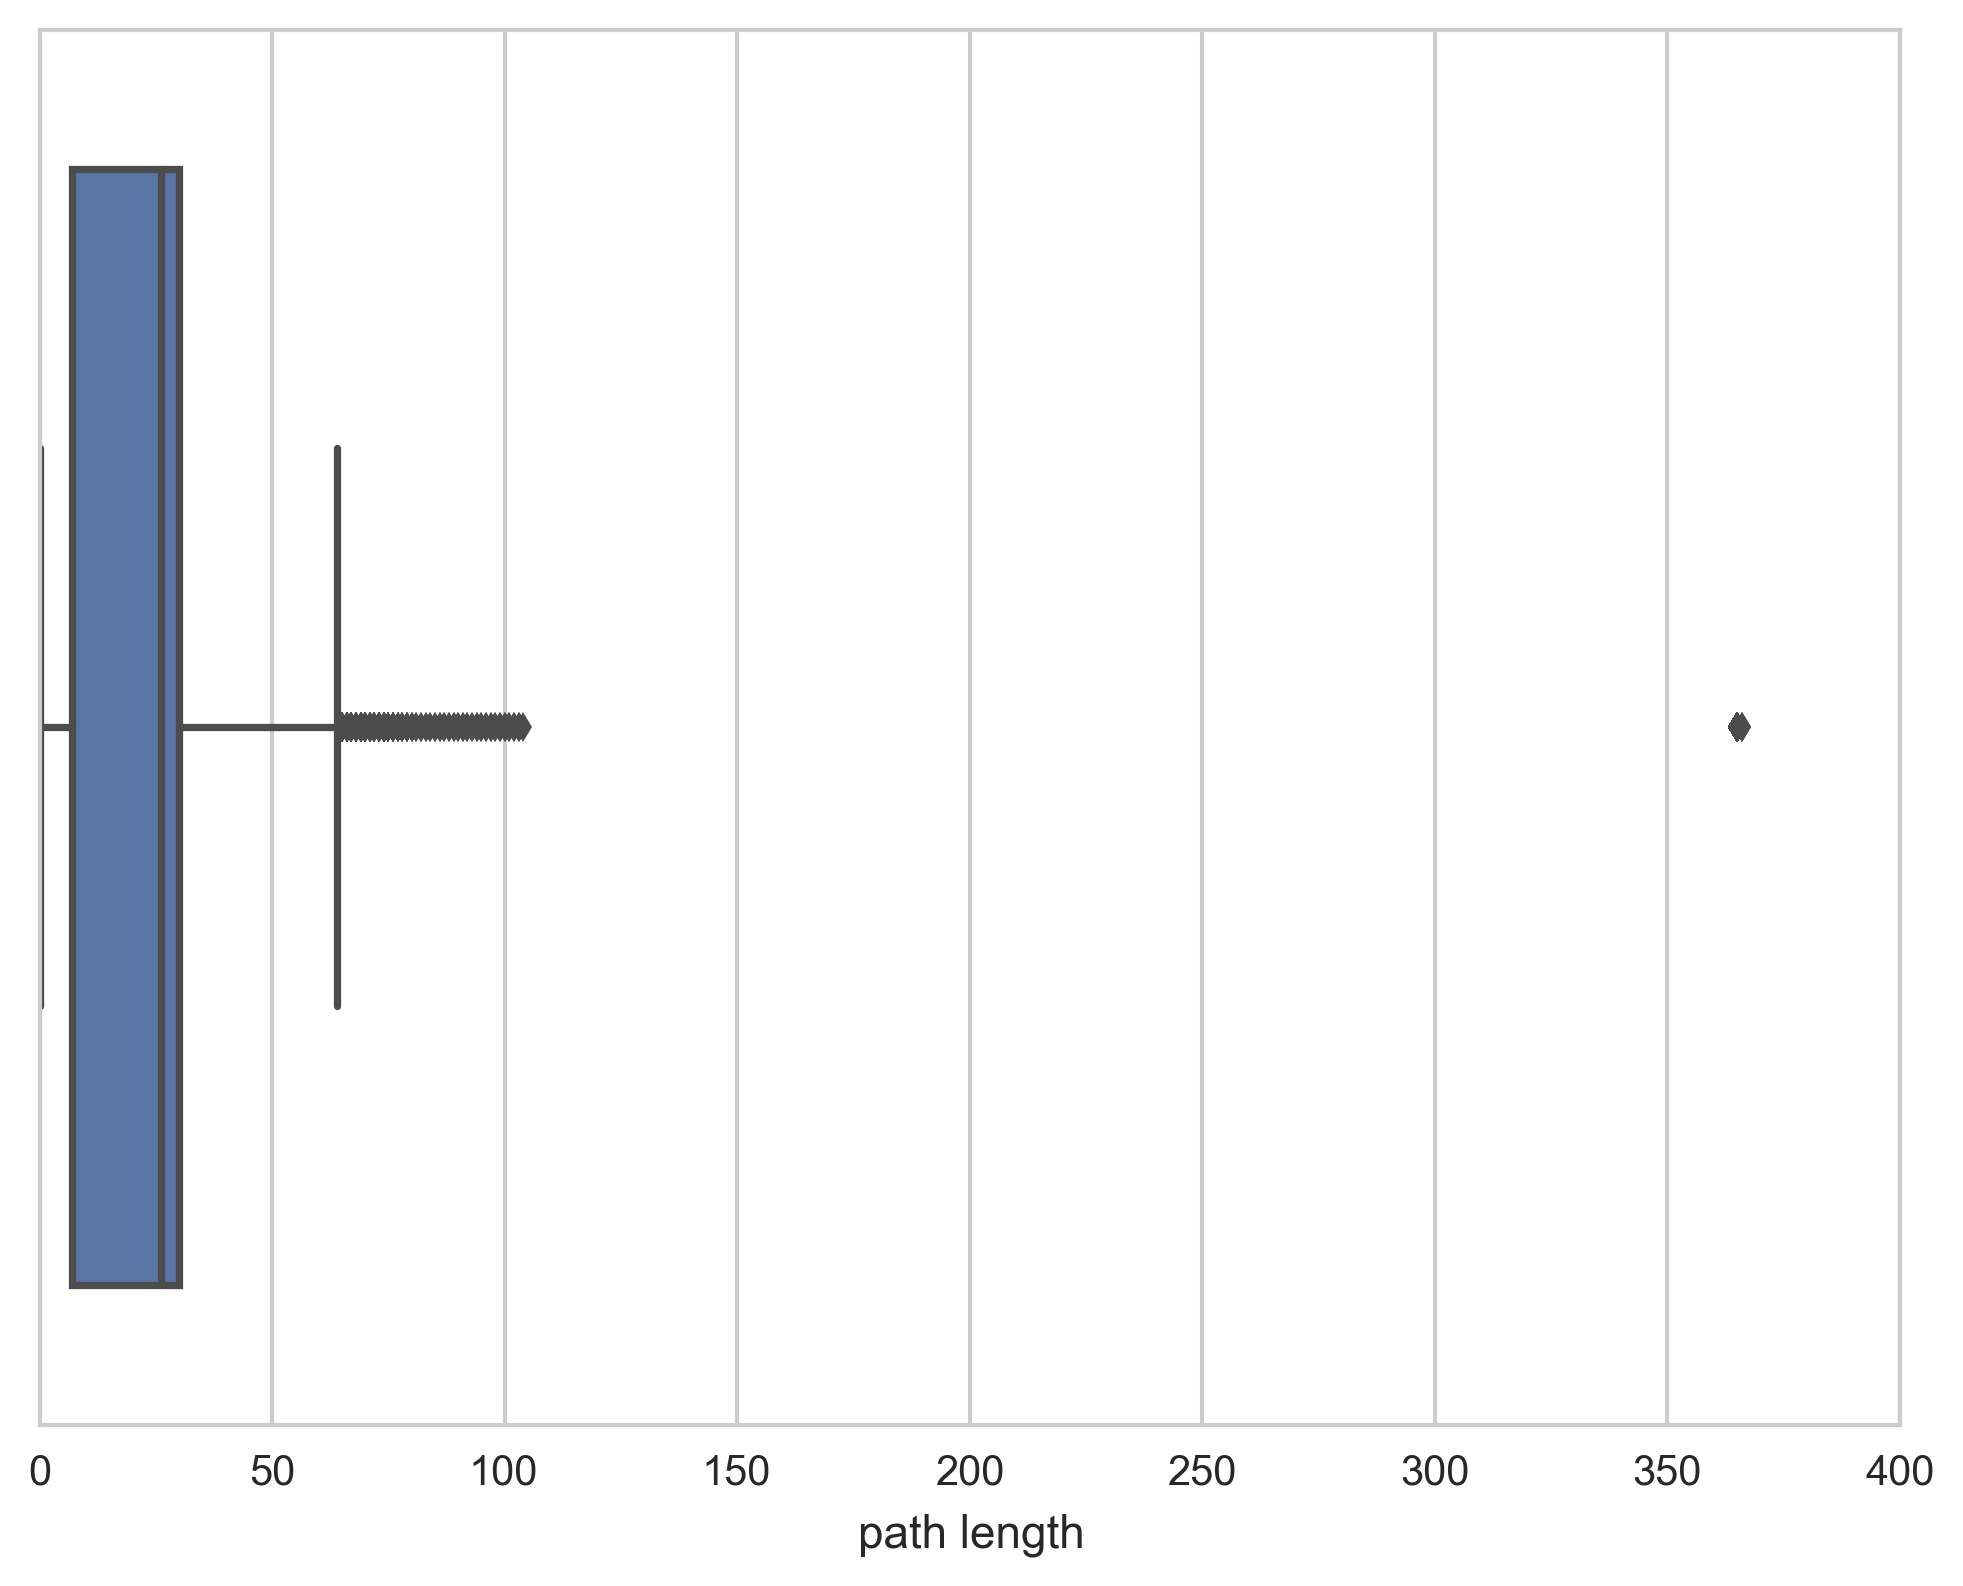
\includegraphics[width=\columnwidth]{graphics/path_lengths_boxplot.png}
  \caption{
    \textbf{Path Length Distribution.}
  }
  The median network depth measured by the number of first links in a path
  is 29. The 365 cycle for ``Orthodox'' liturgics is the outlier to the right, while
  other historical articles about ``Scotland,'' ``UK'' and so on are slightly outside
  the third quartile. More than $75\%$ of articles have path lengths between 
  $0$ and $50$ links.

  \label{fig:Path Length Distribution}
\end{figure}

Of the 11 million articles, 5.5 million had an invalid link or linked back to the same article, yielding a path length of zero. 
This roughly corresponds to the official number of articles on Wikipedia: 
$~4.7$ million as of November 2014---approximately half of the 11 million 
articles in the XML dump are redirects or disambiguations, not full articles.
The most common path length is 29, with an interquartile range of 4---path length
is typically between 26 and 29 articles.
As a distribution, more than $75\%$ of articles have a path length below 
$50$ first links 
while a few temporally organized paths exceed 50 links 
(see figure~\ref{fig:Path Length Distribution}). 



\subsection{Traversal Visits}

As a distribution, the number of traversal visits by article appears to follow a decaying power law. 
The majority of articles have fewer than 30 traversal visits and
first link references accumulate at a few articles.
Specifically, $99.76\%$ of articles have fewer than $100$ traversal visits; nearly $80\%$ have none. 
Meanwhile, the highest ranking 30 articles have an extremely disproportionate number of traversal visits.

\begin{figure}[tp!]
  \centering	
  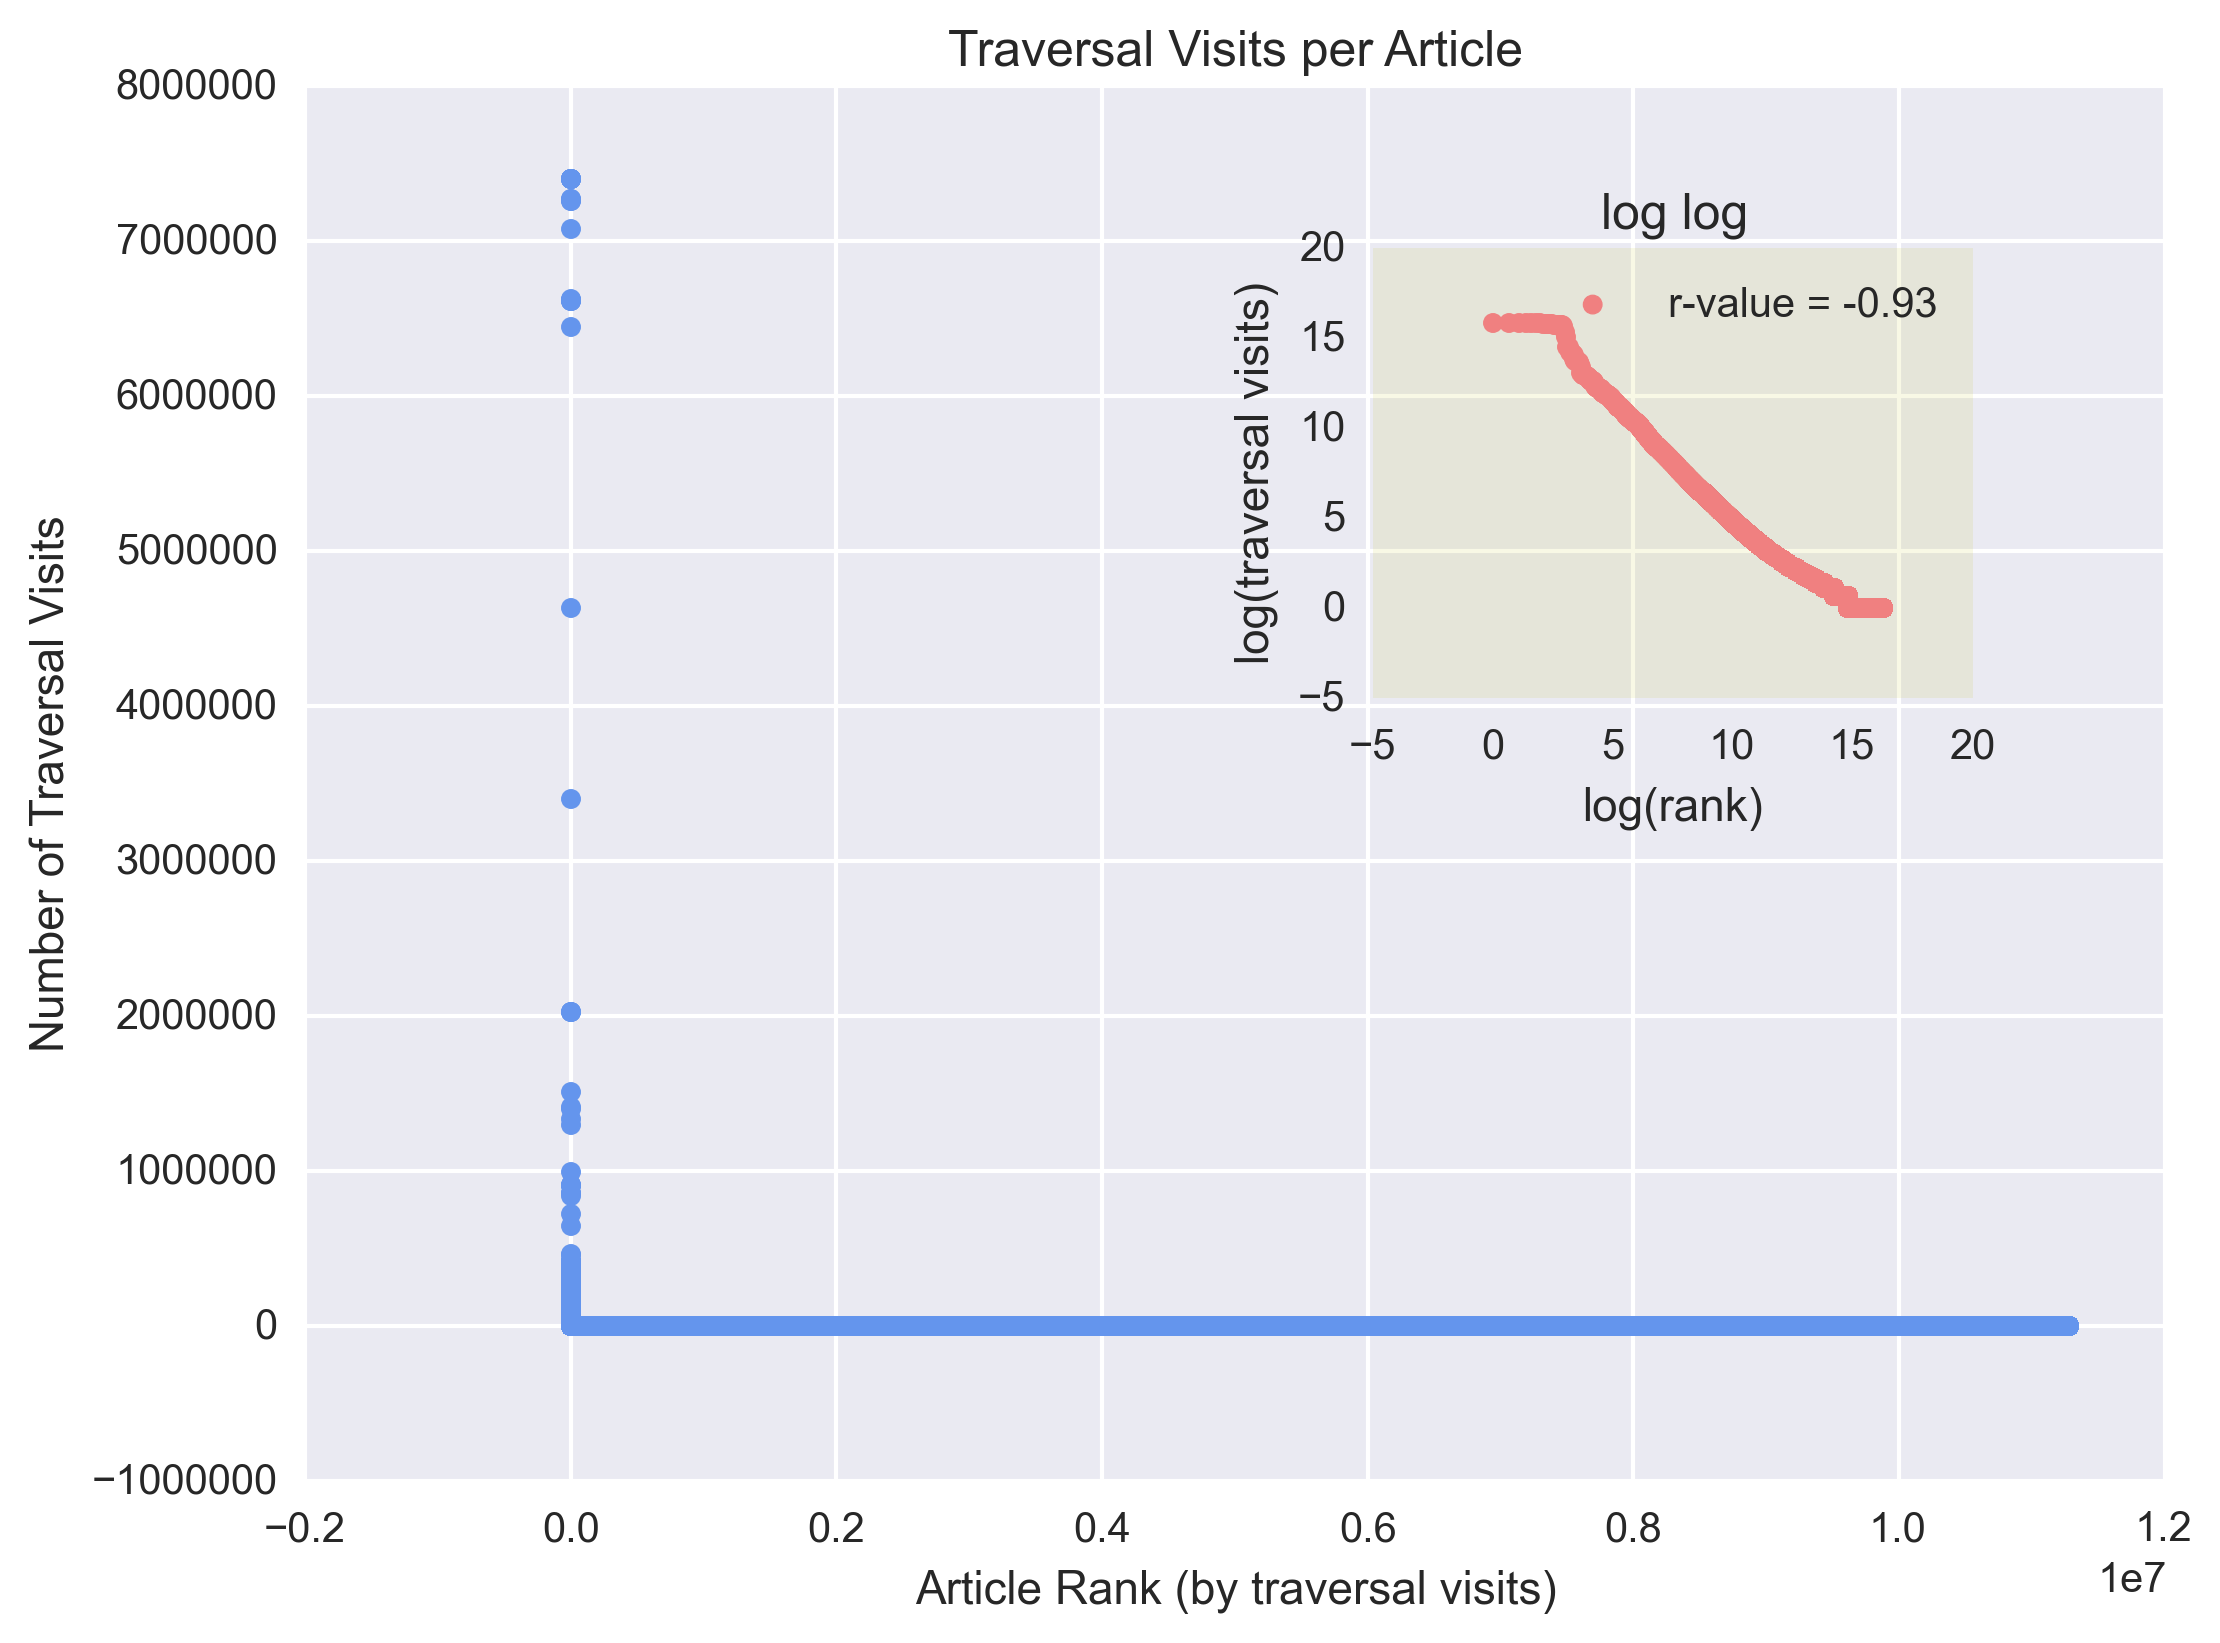
\includegraphics[width=\columnwidth]{graphics/traversals_per_article.png} 
  \caption{
    \textbf{Distribution of Traversal Visits.}
  }
  We fit the distribution to a linear log-log model by considering the log (base 10) transformed rank of each article against log (base 10) transformed the number of traversal visits. 
  The model explains $86\%$ of the variation in the data, yielding an r-value of $-0.93$ 
  and a power law exponent of $-0.64$. The horizontal flattening around the highest
  ranking articles is a result of the cyclic structure (see discussion on cycles).
  \label{fig:Distribution of Visits}

\end{figure}

In Fig., we show a log-log plot for the entire dataset:traversal visits against rank. 
We observe a strong linear fit, with a Pearson's Correlation Coefficient of -.93 and 
a power-law exponent of $-0.636$. A handful of the highest ranking articles contain a disproportionate number of traversal visits, while most have none. The skew in the distribution is not terribly surprising when considering the heuristic of how the links flow: from specific to general. 


\begin{figure}[tp!]
  \centering	
  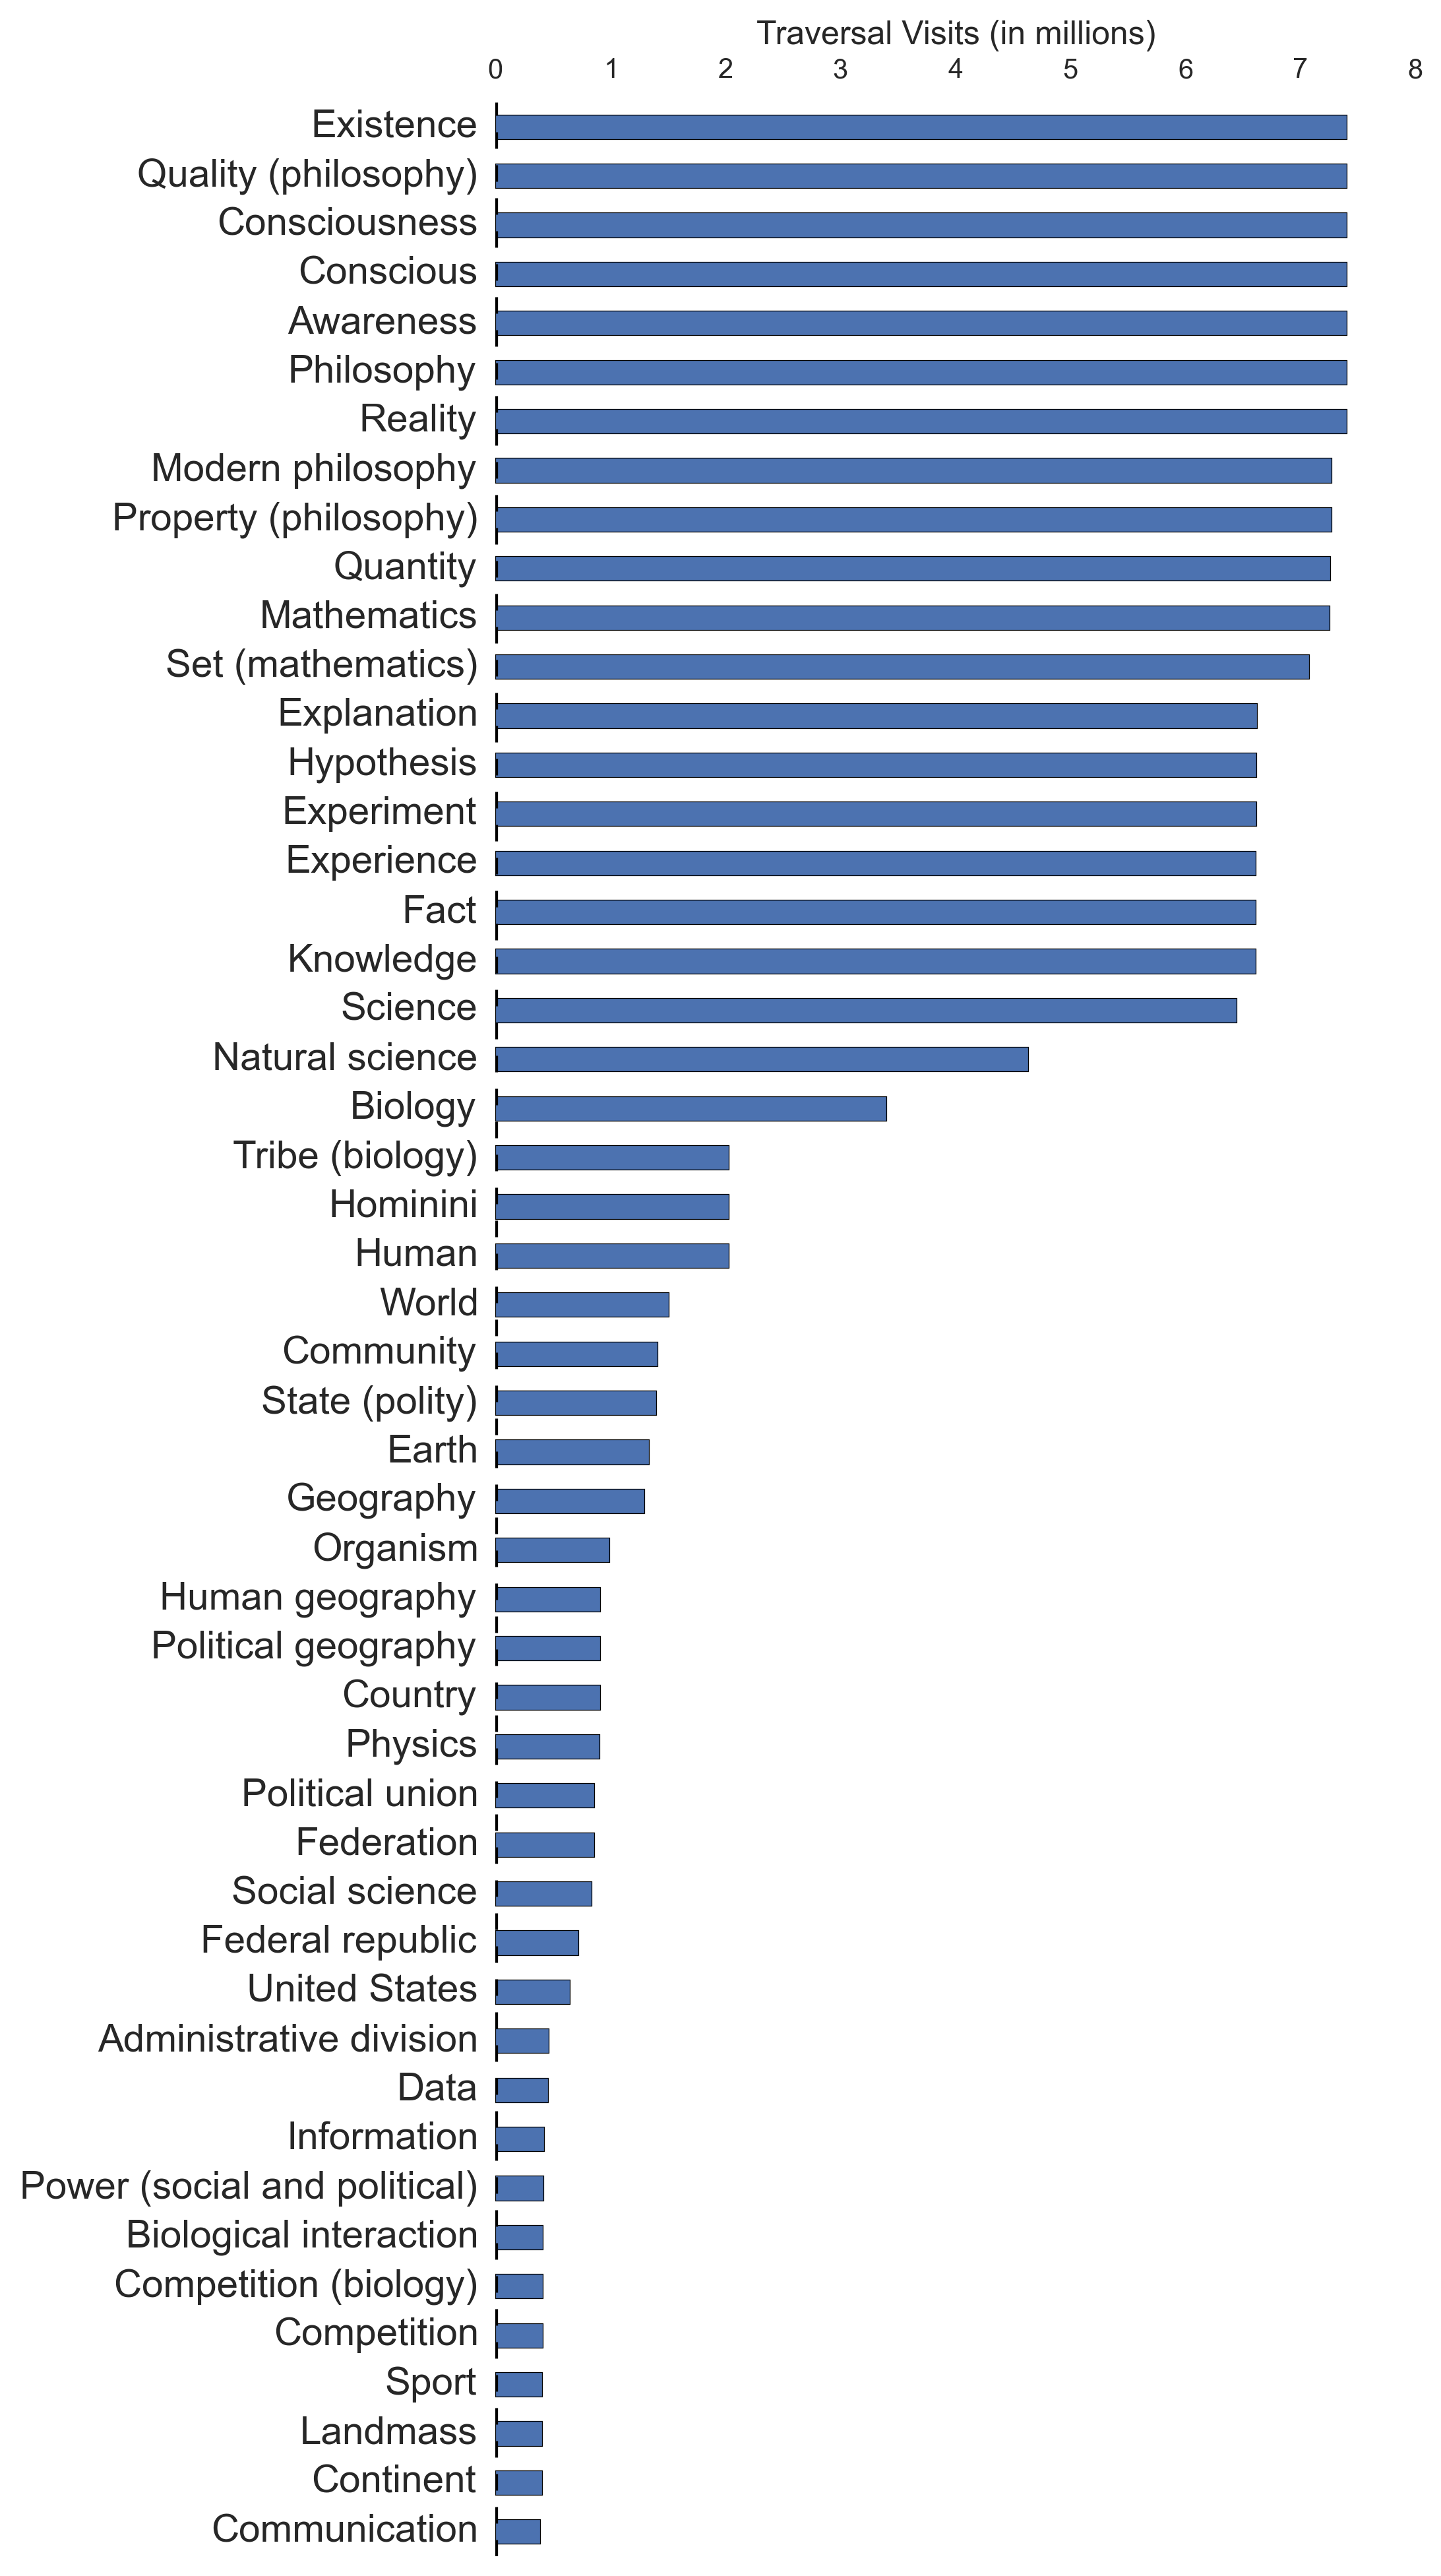
\includegraphics[width=\columnwidth]{graphics/articles_ranked.png}
  \caption{
    \textbf{Highest ranking articles by number of traversal visits.}
  }
  We compute the number of traversal visits for each article in the FLN (see 
  Traversal Algorithm section for details). In doing so, we can rank each article
  by the accumulation of first links. Articles with a greater number of traversal visits
  mark greater points of first link accumulation. The highest ranking articles by traversal visits reveal where the greatest accumulation occurs.
  \label{fig:highest visits}
\end{figure}



\subsection{Network Cycles}

We first identified 2-cycles, meaning a pair of articles with first link pointing to one another.
Of the 11 million articles, 84,000 are 2-cycles. 
The highest ranking 2-cycles by traversal visits tend to be synonyms (or nearly so) rather than distinct, yet connected ideas:
``Health Care'' and ``Medical Case Management,'' ``Broadcasting House,'' and ``BBC,'' ``Secondary Education'' and ``Secondary School'' 
(see Fig.~\ref{fig:2-cycles}).

\begin{figure*}[tp!]
  \centering	
  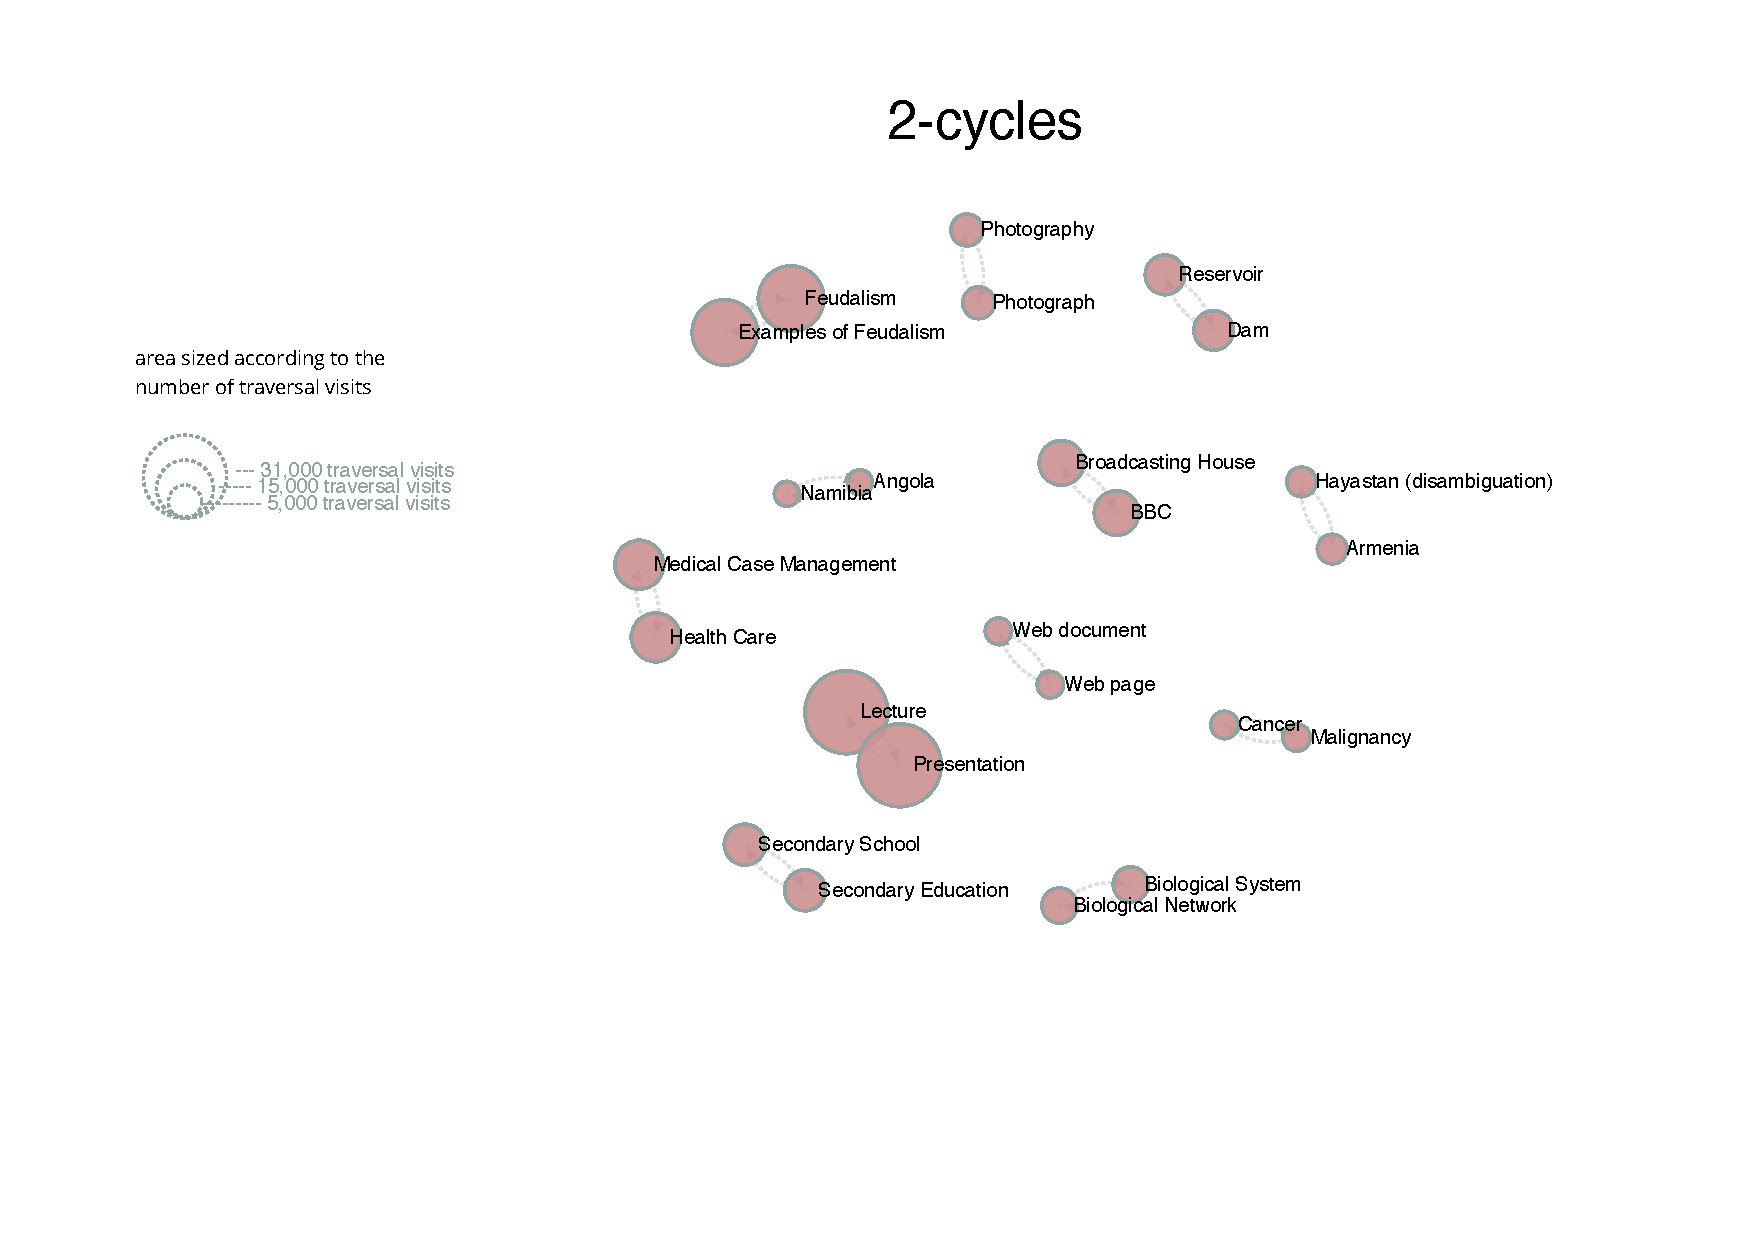
\includegraphics[width=\textwidth]{graphics/2_cycles.pdf}
  \caption{
    \textbf{Highest ranking 2-cycles.}
    We identify pairs of articles whose first links point to one another, forming
    a 2-cycle. We then rank each pair of articles by the total number of 
    traversal visits to gauge the most referenced groups of two articles linked
    to each other. The area of the circles in the figure indicates the number of traversal visits. We find 2-cycles often capture synonyms or articles representing nearly the 
    same concepts as opposed to distinct ideas.
  }
  \label{fig:2-cycles}
\end{figure*}

Outside of the highest ranking 2-cycles, the typical 2-cycle signals a connection between distinct, yet very closely related ideas. 
We also observe link patterns such as inventor to product (``Voere'' to ``VEC-91''), event to organizer (``Poetry Bus Tour'' to ``Weave Books''), and book to author (``Anatomy of Britain'' to ``Anthony Sampson'').

Similarly, 3-cycles capture a synonymous or close relation among 3 articles: ``Tree of life (Biology),'' ``Tree of life (disambiguation),'' 
and ``Tree of life''; ``Cinema of India,'' ``Indian Cinema,'' and ``Telugu Cinema''
(see figure~\ref{fig:3-cycles}).
Once we extend our cycle size beyond a length of 6 however, 
``Philosophy'' along with the remaining list of high ranking articles by traversal visits dominate.
The longest cycle in the network spans 365 articles of Eastern Orthodox Liturgics for each calendar day.
Other lengthy cycles span 60--75 articles including collections of articles on national histories such as ``Japanese Eras'' 
or judicial bodies such as the ``Legislative Assembly of Ontario.''

\begin{figure*}[tp!]
  \centering	
  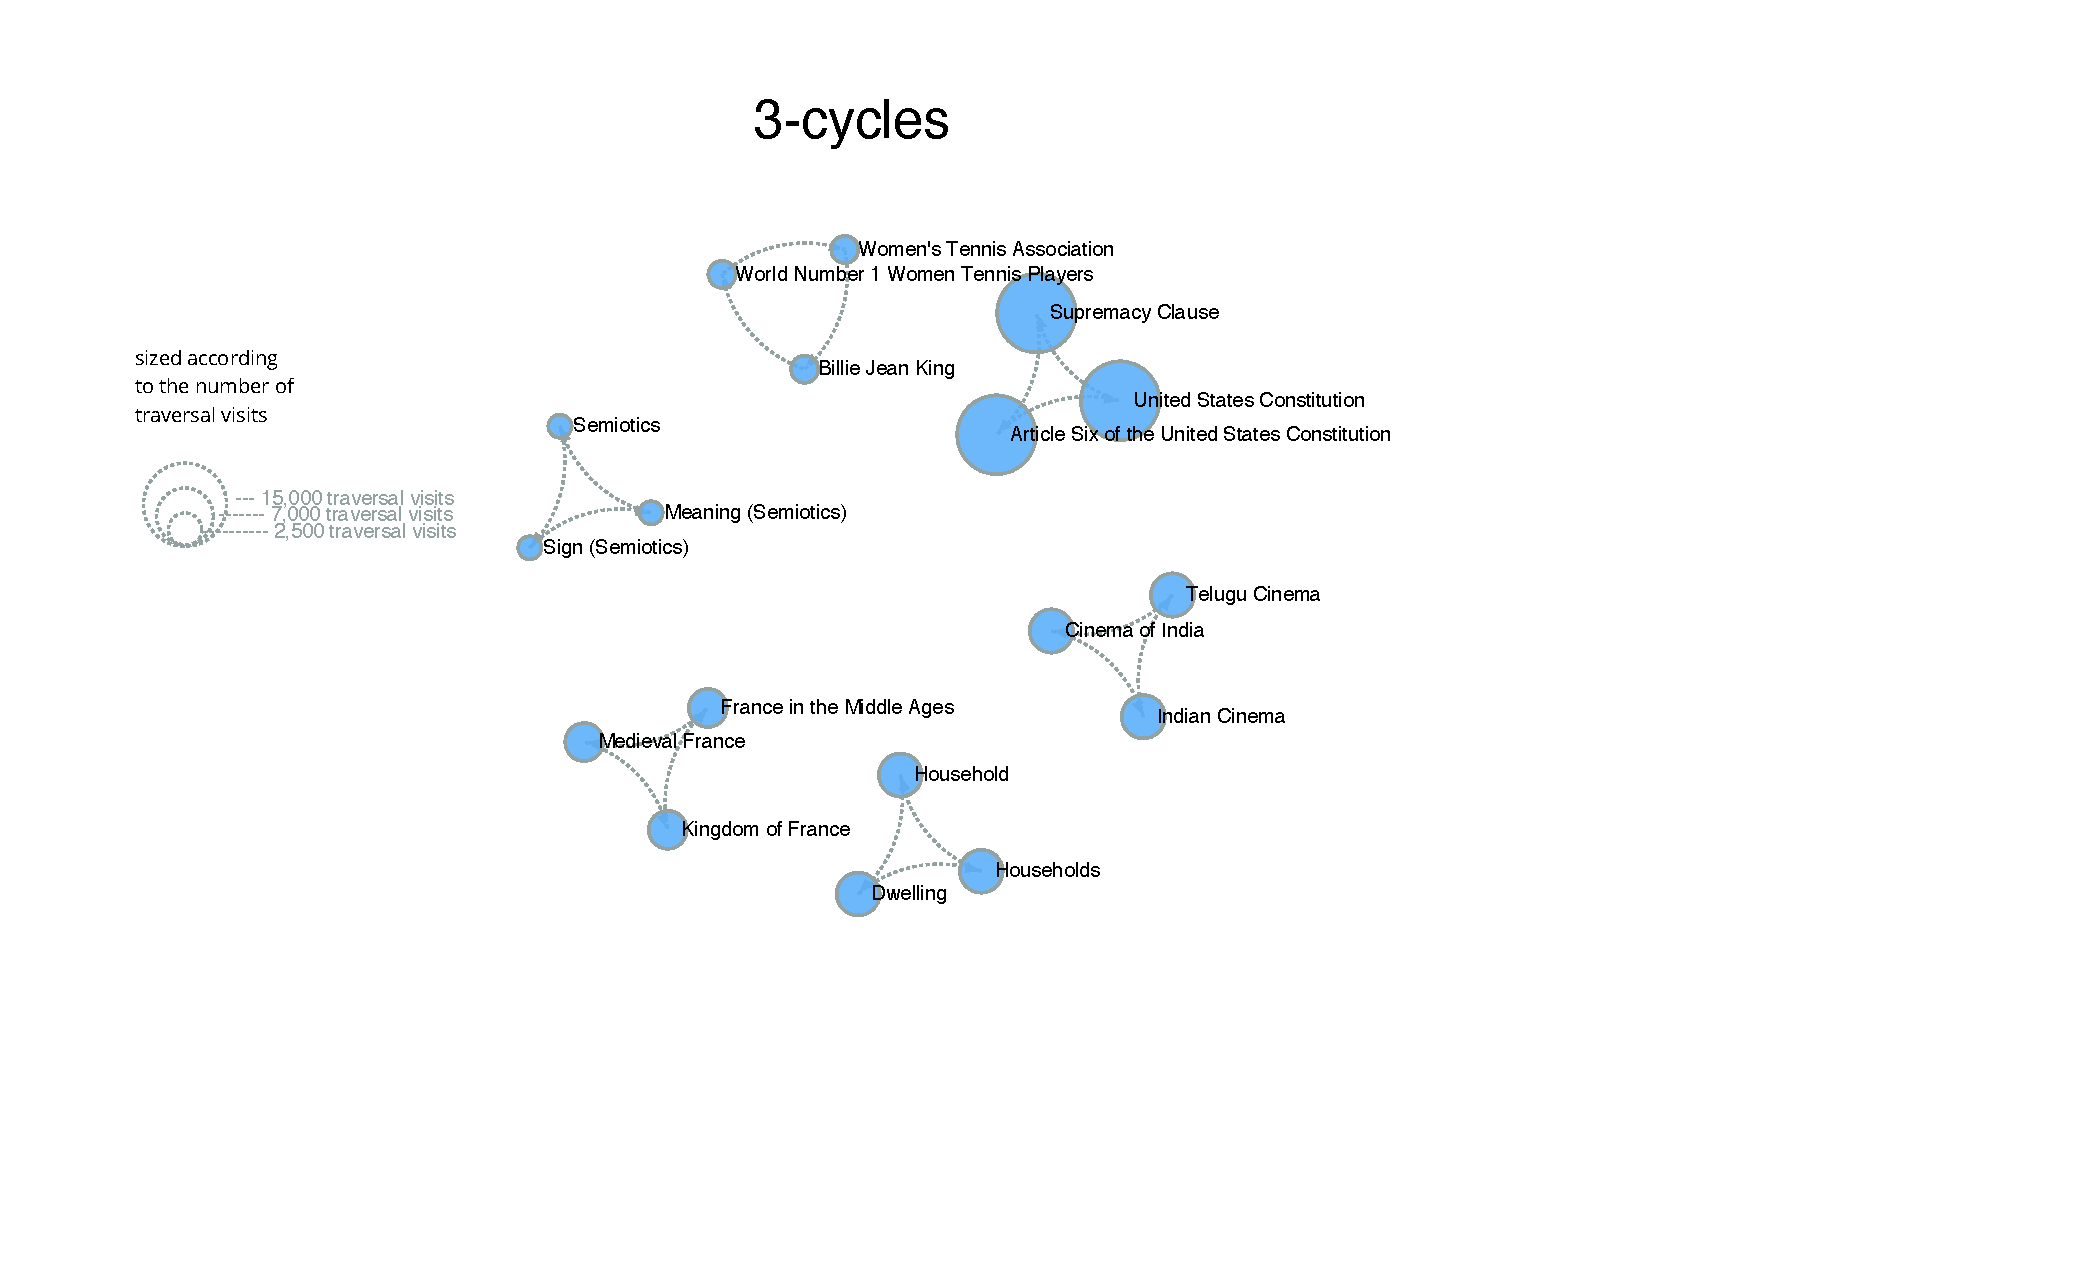
\includegraphics[width=\textwidth]{graphics/3_cycles.pdf}
  \caption{
    \textbf{Highest ranking 3-cycles.}
    We identify groups of three articles whose links form a 3-cycle with the 
    last article in the group linking back to the first article.
    We rank each 3-cycle by the total number of traversal visits to gauge
    the most referenced group of three linked articles. 
    The area of the circles in the figure indicates the number of traversal visits. 
  }
  \label{fig:3-cycles}
\end{figure*}






\subsection{Basins}

We can group articles lying on the same path to identify {\it basins}: 
a group of path-connected articles.
Since cycles identify only groups of articles with a closed set of links, 
we additionally measure and rank basins to capture groups of closely related
articles branching outside of a cycle into the rest of the FLN.
We rank basins by the total number of traversal visits for each article in the path. 
Akin to river networks, these basins are areas of accumulation with a path 
flowing outwards to the rest of the FLN.

The highest ranking basins by the number of traversal visits are groups of articles
around ``Philosophy.'' 
The highest ranking paths include branches of philosophy flowing through 
``Awareness,'' ``Existence,'' and ``Consciousness'' to ``Philosophy.'' Other paths
include concepts around ``Mathematics,'' ``Scientific,'' ``Experiments,'' 
``Biology,'' and ``Fact.''
These paths link many specific articles to ``Philosophy,'' each funneled through a particular domain.

Excluding basins around ``Philosophy,'' we find other basins around 
foundational concepts such as ``Community,'' ``Landmass,'' ``Federal Government,'' 
``Presentation,'' and ``Belief System.'' 
The basins around each of these foundational notions are 
various paths containing related articles. For example around 
``Community'' we find basins
flowing from ``United States'' to ``Federal Republic'' to ``Political Union'' to ``State'' culminating at ``Community''; we also find basins flowing from 
``Public Policy'' to ``Executive (government)'' to ``Government'' to ``State'' and then 
to ``Community''; we also find paths flowing through a similar chain beginning
with ``Democracy,'' another beginning with ``Constitution,'' another at 
``Dictatorship,'' and so on. The ideas build from specific means of organizing
a community (or society) and then build up to ``Community.'' 
Other basins around landmass for example begin at specific geographical regions
such as ``Eastern Europe'' building up to ``Continent'' and finally ``Landmass''.


\subsection{Traversal Funnels}

To analyze the influence an article exerts in shaping the 
structure of the FLN, we compute the number of traversal funnels for each.
Articles directing more paths exert a greater influence over the structure
of the FLN by increasing the accumulation of first links
on a particular path. By measuring traversal funnels, we distinguish between an article that simply happened to fall within a cycle from an article funneling 
many first links.

Ranking articles by the number of traversal funnels we find 
``Philosophy'' to be by far the highest-ranking article with 
$7.37$ million paths
(see figure~\ref{fig:Funnels}).
\begin{figure*}[tp!]
  \centering	
  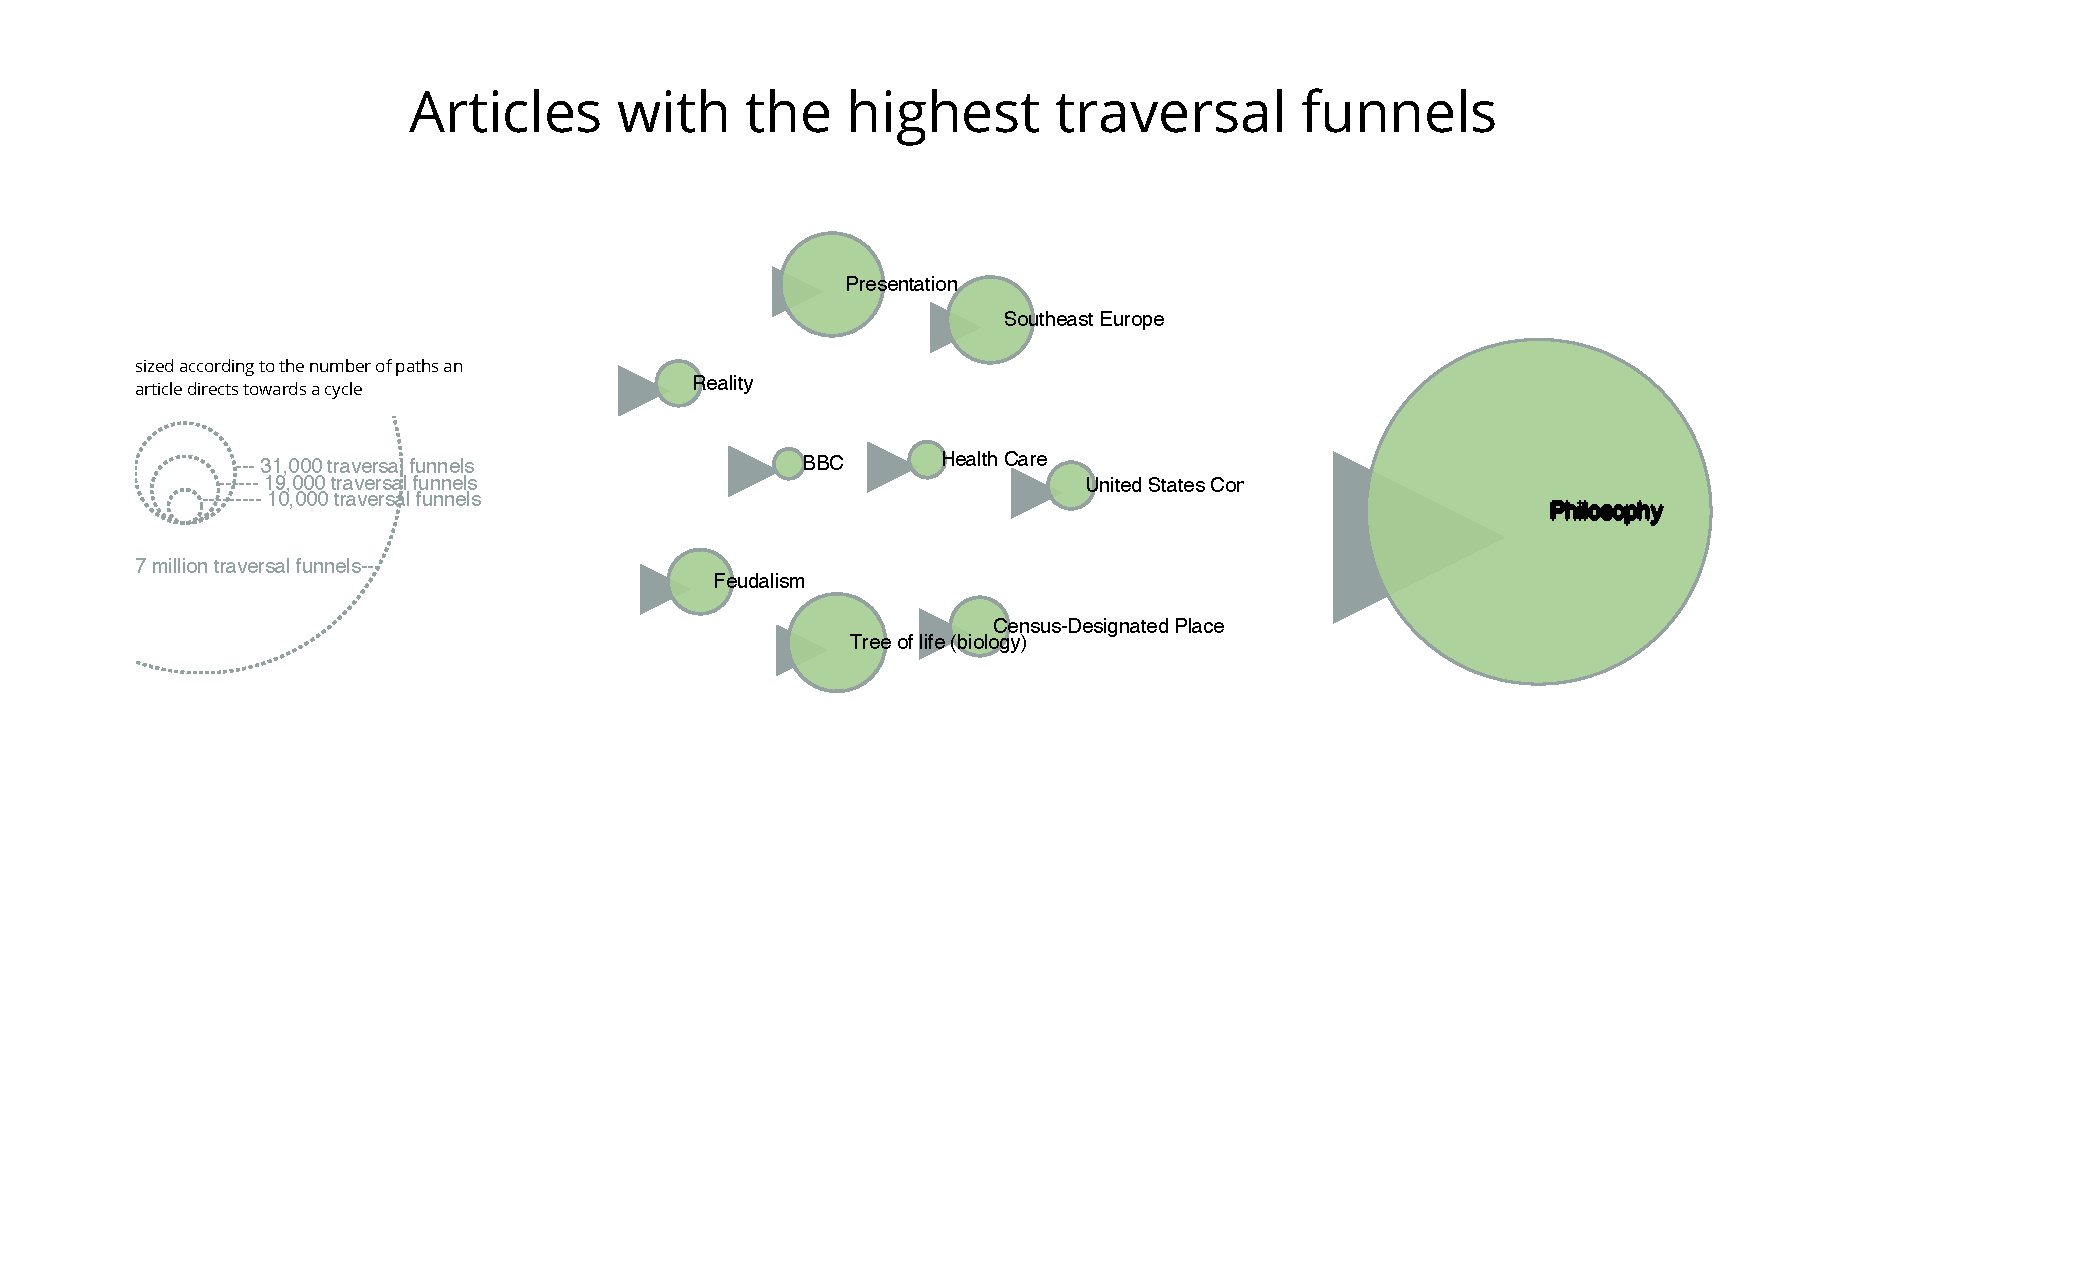
\includegraphics[width=\textwidth]{graphics/funnels.pdf}
  \caption{
    \textbf{Funnels.}
    We represent the highest-ranking articles by the number of traversal 
    funnels to gauge the influence each article exerts in shaping the 
    structure of the FLN. 
    The area of each circle is sized in proportion to the number of 
    traversal funnels each article has. 
    We find ``Philosophy'' exerts an overwhelming proportion
    of the influence, with other abstract notions and topical concepts ranking
    next.
  }
  \label{fig:Funnels}
\end{figure*}
Of any article, the number of traversal funnels Philosophy holds exceeds 
all others by more than two orders of magnitude.
The ``Philosophy'' cycle which contains ``Existence,'' ``Awareness,'' ``Reality,'' 
and similar articles accumulates the overwhelming proportion of its 
references through ``Philosophy'': $7.37$ million of the $7.4$ million references
are funneled through ``Philosophy''.
Second on the list of highest-ranking articles by traversal funnels is 
``Presentation'' with only $30$ thousand paths. Similarly abstract 
ideas also rank highly such as ``Tree of life'' (30 thousand), 
``Reality'' (13 thousand), and ``Jurisdiction'' (3 thousand).

Many high-ranking articles are remarkably topical, culturally and politically important ideas.  For example, ``Health Care'', a recently high-contested legislative topic appears high on the list---Google trends indicates an uncharacteristic spike in search frequency between August, 2009 and February, 2010.
Other high ranking articles include key historical events such as the ``Cold War'' or critical scarce resource with recent 
media discussion such as ``Fossil Fuel''. 
The highest-ranking list also includes ``Hip Hop,'' ``Cancer,'' and ``Web Page''.
\begin{figure}[tp!]
  \centering	
  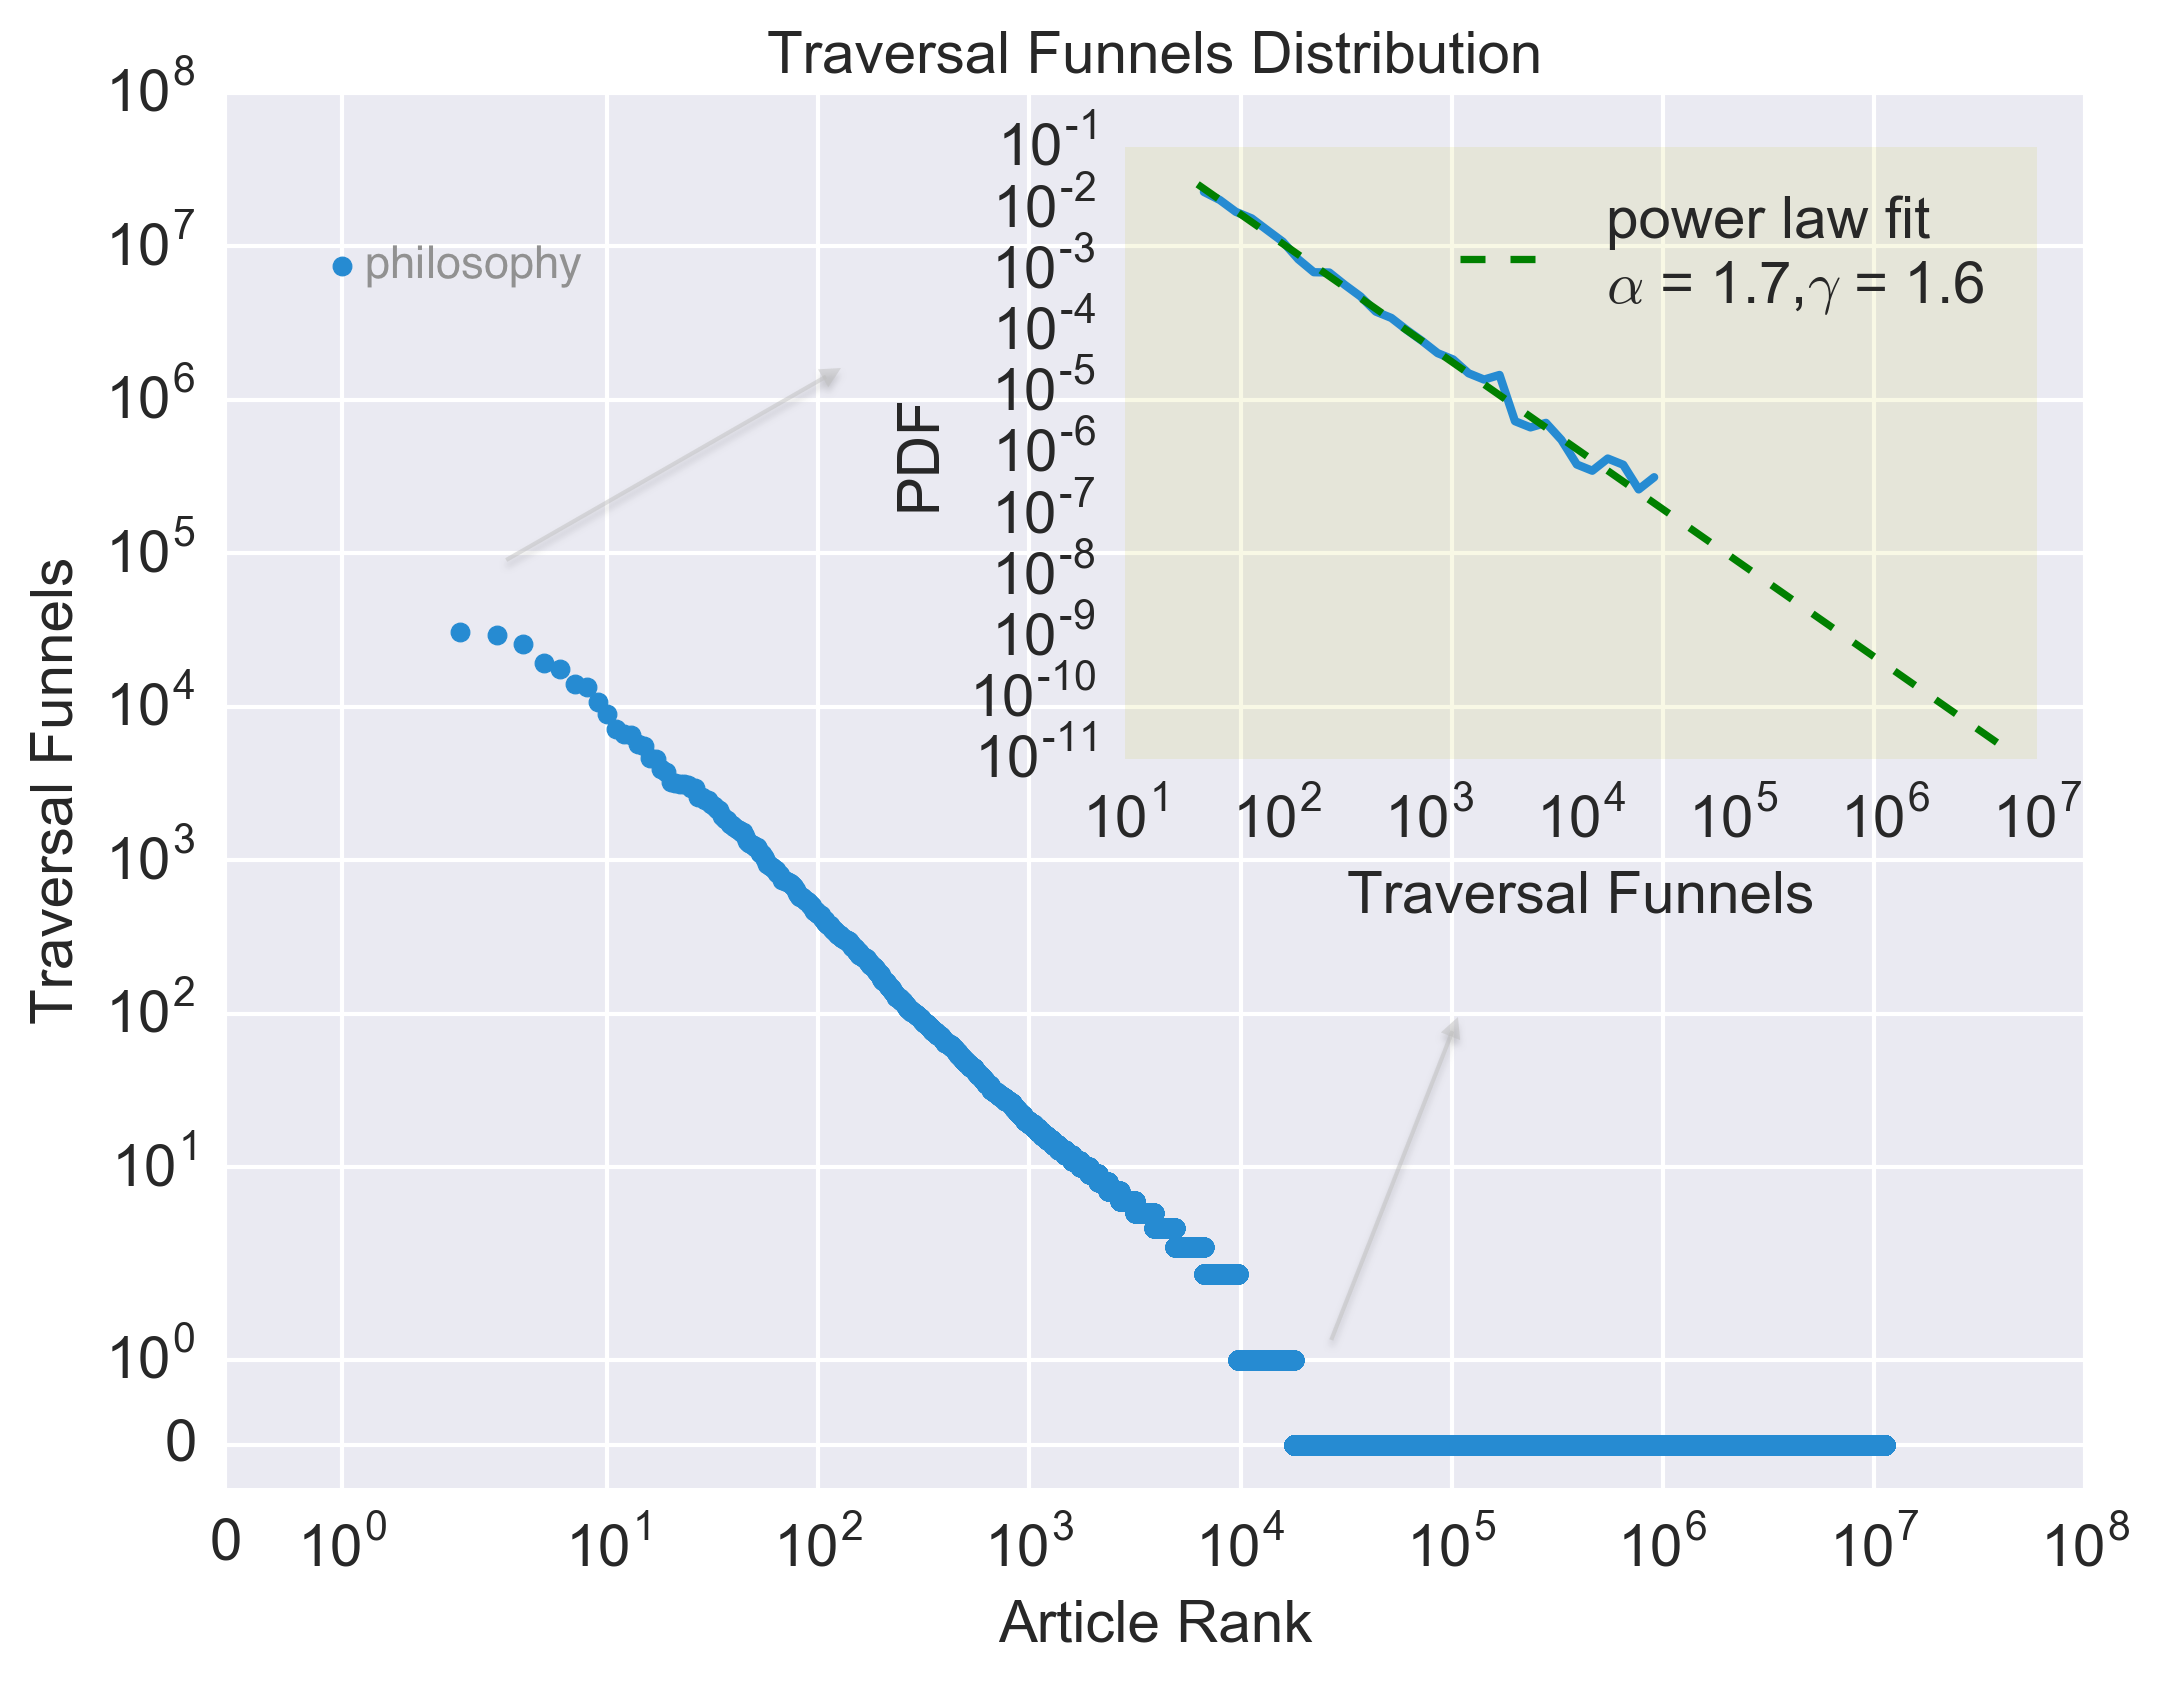
\includegraphics[width=\columnwidth]{graphics/funnels_distribution.png}
  \caption{
    \textbf{Distribution of Traversal Funnels.}
  We fit the distribution with a linear log-log model by considering the log (base 10) transformed rank of each article against log (base 10) transformed the number of traversal funnels. 
  We find two regimes with the top regime (log(rank) < 4) 
  well-explained by a linear fit, yielding an r-value of $-0.99$ and a 
  power-law exponent of $-1.08$. The top regime 
  explains the distribution of traversal funnels for the $17, 821$ 
  articles with at least one traversal funnel. The bottom 
  horizontal regime corresponds to the more than $99\%$ of articles
  which hold zero traversal funnels.
  }
  \label{fig:Funnels Distribution}
\end{figure}

As a distribution, we find few articles influence the structure of the 
FLN. Only $17, 821$ articles have one or more traversal funnels, leaving
an more than $99\%$ with none---most articles are recipients of 
the references flowing through the articles with at least one traversal funnel.
When fit to a log-log linear model we find the $99\%$ of articles with zero
traversal funnels form one regime (with log(rank) less than 4).
The top regime, corresponding to the $17, 821$ articles with at least one 
traversal funnel strongly fits a linear model with an r-value of $-0.99$. 
The resulting power-law exponent is $-1.08$. Even within the few articles
influencing the structure of the FLN, only a handful of these exert most of the 
control. 

\end{document}
